\UseRawInputEncoding
\RequirePackage{setspace}		% Hinzugefügt: Entfernt Warnungen wenn \footnote benutzt wird, Manuel Schwartz 2016.03.20

%%% Abschlussarbeiten am IRS - LaTeX-Vorlage %%%
% --- %
% Bei einer englishen Arbeit die nachfolgenden Zeilen vertauscht ein - und auskommentieren

%\documentclass[pdftex,english]{irsdiplom}
%\usepackage{etoolbox}
%\newbool{symbol_english}
%\setbool{symbol_english}{true}

%\documentclass[pdftex]{irsdiplom}
\documentclass[pdftex,english]{irsdiplom}
\usepackage{etoolbox}
\newbool{symbol_english}
\setbool{symbol_english}{true}

% --- %

% Creates a footnote style rule, which can be used in captions
\makeatletter
\def\footnoterule{\\[-1.5mm]  \rule{5cm}{0.1pt} \\}
\makeatother


% Literaturverzeichnis
\usepackage{bibgerm}

\usepackage[font=scriptsize]{caption}

% Tabellen
% 28.05.2020
% this package is for having a sideways table
\usepackage{rotating}
% For gray midrules
\usepackage[table]{xcolor}
\usepackage{booktabs}
%\usepackage{array}
\usepackage{tabularx}							% Neues package für Tabellen, Manuel Schwartz 2016.02.18
\renewcommand\tabularxcolumn[1]{m{#1}}
\usepackage{supertabular}

% Mathematik
\usepackage{nicefrac}							% Neues package für Brüche, Manuel Schwartz 2016.02.20
\usepackage{siunitx}							% Neues package zur Angabe von Maßeinheiten, Manuel Schwartz 2016.03.05
\usepackage{amssymb}
\usepackage{amsmath}
%\usepackage{gensymb}
%\usepackage{theorem}
%\usepackage[thinspace,thickqspace]{SIunits}
%\usepackage{trsym} 	% Laplace-Hantel

% Hier können weitere Umgebungen erzeugt werden, z.B. Satz, lemma etc.
%	\newtheorem{'Aufruf im Quelltext'}{'Name im Quelltext'}['Numerierung auf Ebene: chapter, section, subsection, ...]		% Ergänzt Manuel Schwartz 2016.02.20
\newtheorem{definition}{Definition}[chapter]
\newtheorem{regel}{Regel}[chapter]

% Grafiken
%\usepackage{subfigure}						% Geaendert von \package{subfig}: Neues package für Mehrere Grafiken nebeneinander, Manuel Schwartz 2016.02.18
\usepackage{tikz}
\usetikzlibrary{external}
%\tikzexternalize[mode=list and make]			% Beim Einkommentieren werden die Bildausgaben von Tikz unterdrückt (deutlich schnelleres Kompilieren), Oliver Stark 2016.09.02

% Sprache und Schrift
\usepackage[utf8]{inputenc}
\usepackage{lmodern}	%% Ersetzt das veraltete \package{caption} (Alte Warnung) aus irsdiplom.cls Zeile 1256 bis 1265
\newcommand{\changefont}[3]{
\fontfamily{#1}\fontseries{#2}\fontshape{#3}\selectfont}
% Diese Optionen von Caption machen die Namen (Abbildung, Tabelle) sowie deren Nummer fett und in footnotesize
%\usepackage[labelfont=bf,textfont=footnotesize]{caption}

% Richtiges Schreiben von Matlab und Simulink (Gerade in Small Caps)
\newcommand{\Matlab}{{\rm \sc Matlab}}
\newcommand{\Simulink}{{\rm \sc Simulink}}
%\newcommand{\initialisiert}{{\rm \sc initialisiert}}
%\newcommand{\Stromintegration}{{\rm \sc Stromintegration}}

% Worttrennung
\hyphenation{Strom-integration}




% Quellcode
%
% Hier wird die Matlab Syntax für listings eingeführt
% Syntax:
%
% \begin{lstlisting}
% 	Quellcode direkt aus Matlab hier her kopieren
%	\end{lstlisting}
%
% ---------------------------------------------------
\usepackage{listings} \lstset{numbers=left, numberstyle=\tiny, numbersep=5pt} \lstset{language=Matlab} 
% Umlaute und ß für Codeumgebung, Oliver Stark 2016.09.02
\lstset{basicstyle=\ttfamily}
\lstset{literate=%
	{Ö}{{\"O}}1
	{Ä}{{\"A}}1
	{Ü}{{\"U}}1
	{ß}{{\ss}}2
	{ü}{{\"u}}1
	{ä}{{\"a}}1
	{ö}{{\"o}}1
} 

% Farben
\usepackage{color}
\definecolor{mygreen}{rgb}{0,0.6,0}
\definecolor{mygray}{rgb}{0.5,0.5,0.5}
\definecolor{mymauve}{rgb}{0.58,0,0.82}

\lstset{ %
  backgroundcolor=\color{white},   		% choose the background color; you must add \usepackage{color} or \usepackage{xcolor}
  basicstyle=\footnotesize,        					% the size of the fonts that are used for the code
  breakatwhitespace=false,         			% sets if automatic breaks should only happen at whitespace
  breaklines=true,                 								% sets automatic line breaking
  captionpos=b,                    								% sets the caption-position to bottom
  commentstyle=\color{mygreen},    	% comment style
  deletekeywords={...},            						% if you want to delete keywords from the given language
  escapeinside={\%*}{*)},          					% if you want to add LaTeX within your code
  extendedchars=true,              						% lets you use non-ASCII characters; for 8-bits encodings only, does not work with UTF-8
  frame=single,                    								% adds a frame around the code
  keepspaces=true,                 						% keeps spaces in text, useful for keeping indentation of code (possibly needs columns=flexible)
  keywordstyle=\color{blue},       				% keyword style
  language=Octave,                 						% the language of the code
  morekeywords={*,...},            						% if you want to add more keywords to the set
  numbers=left,                    									% where to put the line-numbers; possible values are (none, left, right)
  numbersep=5pt,                   						% how far the line-numbers are from the code
  numberstyle=\tiny\color{mygray}, 		% the style that is used for the line-numbers
  rulecolor=\color{black},         						% if not set, the frame-color may be changed on line-breaks within not-black text (e.g. comments (green here))
  showspaces=false,                						% show spaces everywhere adding particular underscores; it overrides 'showstringspaces'
  showstringspaces=false,          				% underline spaces within strings only
  showtabs=false,                  							% show tabs within strings adding particular underscores
  stepnumber=2,                    							% the step between two line-numbers. If it's 1, each line will be numbered
  stringstyle=\color{mymauve},     			% string literal style
  tabsize=2,                       										% sets default tabsize to 2 spaces
  title=\lstname                   									% show the filename of files included with \lstinputlisting; also try caption instead of title
}
% ---------------------------------------------------

%% Packages "german" und "graphicx" werden bereits mit der Klasse "irsdiplom" geladen
\graphicspath{{./img/}}	%% Geaendert, Manuel Schwartz 2015.10.13
%% Einbinden des .tex-files, welches die Angaben wie Titel, Autor, etc. enth"alt.
%% M"oglichst Leerzeichen im Dateinamen vermeiden! Die Endung .tex wird automatisch erg"anzt.
%%%
% Aenderung, der Befehl \changefont{phv}{m}{n}{} wurde eingeführt damit im restlichen
% Dokument \uspackage{lmodern} genutzt werden kann, Manuel Schwartz 2015.10.13
% Soll die Schriftart auf diesen beiden Seiten geändert werden, so muss in irsdiplom.cls
% bei jedem Merker [MerkerMS01] ebenfalls die Schriftart geändert werden
%%%

%% Deckblatt
\author{\changefont{phv}{m}{n}{Jonas Teufel}}
\title{\changefont{phv}{b}{n}{Analysis of Existing Algorithms for the Coordination of Heterogeneous Robotic Teams}}	% Hier bitte beide ausfüllen
\titlem{\changefont{phv}{m}{n}{Analysis of Existing Algorithms for the Coordination of Heterogeneous Robotic Teams}}	% Hier bitte beide ausfüllen

%% Informationen über die Abschlussarbeit
% Nummer und Format der Arbeit
\arbeitnummer{\changefont{phv}{b}{n}{Nummer der Arbeit}}
\arbeittyp{\changefont{phv}{b}{n}{Bachelorarbeit}}		% Hier bitte beide ausfüllen
\arbeittypm{\changefont{phv}{m}{n}{Bachelorarbeit}}		% Hier bitte beide ausfüllen
% Name und Titel des Betreuers
{\betreuer{\changefont{phv}{m}{n}{Esther Bischoff, M.Sc.}} 
{\zweitpruefer{\changefont{phv}{m}{n}{Dr.-Ing. Vorname Nachname}} % Hier bitte ausf�llen
\coop{\changefont{phv}{b}{n}{Name des Unternehmens}} % Für externe Arbeiten
% Anfangs- und Abgabedatum
\startdate{{\changefont{phv}{m}{n}{\!{\!}06.04.2020}}} 		%englisches Datum MM/DD/YYY
\date{{\changefont{phv}{m}{n}{\!{\!}01.07.2017}}}			%englisches Datum MM/DD/YYY
\defensedate{{\changefont{phv}{m}{n}{\!{\!}14.11.2020}}}		
% Für Sperrvermerk hier Abgabedatum + 5 Jahre 				% Für externe Arbeiten
\dateEnd{{\changefont{phv}{m}{n}{\!{\!}01.07.2022}}}		%englisches Datum MM/DD/YYY

% Beschreibung der Aufgabenstellung
\beschreibung{\changefont{phv}{m}{n}{Hier sollte die Aufgabenstellung kurz beschrieben werden...maximal diese Seite, sodass unten noch Platz für die entsprechenden Angaben bleibt}}

% Sonstiges
\keywords{\changefont{phv}{m}{n}{vehicle routing, multi robot coordination, genetic algorithm, computational experiments}}
 % Beispiel: %%%
% Aenderung, der Befehl \changefont{phv}{m}{n}{} wurde eingeführt damit im restlichen
% Dokument \uspackage{lmodern} genutzt werden kann, Manuel Schwartz 2015.10.13
% Soll die Schriftart auf diesen beiden Seiten geändert werden, so muss in irsdiplom.cls
% bei jedem Merker [MerkerMS01] ebenfalls die Schriftart geändert werden
%%%

%% Deckblatt
\author{\changefont{phv}{m}{n}{Jonas Teufel}}
\title{\changefont{phv}{b}{n}{Analysis of Existing Algorithms for the Coordination of Heterogeneous Robotic Teams}}	% Hier bitte beide ausfüllen
\titlem{\changefont{phv}{m}{n}{Analysis of Existing Algorithms for the Coordination of Heterogeneous Robotic Teams}}	% Hier bitte beide ausfüllen

%% Informationen über die Abschlussarbeit
% Nummer und Format der Arbeit
\arbeitnummer{\changefont{phv}{b}{n}{Nummer der Arbeit}}
\arbeittyp{\changefont{phv}{b}{n}{Bachelorarbeit}}		% Hier bitte beide ausfüllen
\arbeittypm{\changefont{phv}{m}{n}{Bachelorarbeit}}		% Hier bitte beide ausfüllen
% Name und Titel des Betreuers
{\betreuer{\changefont{phv}{m}{n}{Esther Bischoff, M.Sc.}} 
{\zweitpruefer{\changefont{phv}{m}{n}{Dr.-Ing. Vorname Nachname}} % Hier bitte ausf�llen
\coop{\changefont{phv}{b}{n}{Name des Unternehmens}} % Für externe Arbeiten
% Anfangs- und Abgabedatum
\startdate{{\changefont{phv}{m}{n}{\!{\!}06.04.2020}}} 		%englisches Datum MM/DD/YYY
\date{{\changefont{phv}{m}{n}{\!{\!}01.07.2017}}}			%englisches Datum MM/DD/YYY
\defensedate{{\changefont{phv}{m}{n}{\!{\!}14.11.2020}}}		
% Für Sperrvermerk hier Abgabedatum + 5 Jahre 				% Für externe Arbeiten
\dateEnd{{\changefont{phv}{m}{n}{\!{\!}01.07.2022}}}		%englisches Datum MM/DD/YYY

% Beschreibung der Aufgabenstellung
\beschreibung{\changefont{phv}{m}{n}{Hier sollte die Aufgabenstellung kurz beschrieben werden...maximal diese Seite, sodass unten noch Platz für die entsprechenden Angaben bleibt}}

% Sonstiges
\keywords{\changefont{phv}{m}{n}{vehicle routing, multi robot coordination, genetic algorithm, computational experiments}}



% =================================================================================================================
% COMMANDS
% This file "Commands.tex" contains all the new command definitions, which were written just for this thesis.
% These commands are for example used in the tables and the mathematics expressions.

% COMPARISON TABLES
% =================
% The following commands are to be used in the comparison tables in the second chapter "literature review"

% This command wraps a few other commands, which are commonly used to init the "table" environment. That is for 
% example centering the content and setting row column spacing
\newcommand{\tableConfig}{\centering \setlength{\tabcolsep}{8pt} \renewcommand*{\arraystretch}{1.3} \scriptsize}

% A shorthand for the checkmark symbol, which is faster to write, because it is being used 
% so much in the comparison tables
\newcommand{\yes}{\checkmark}
\newcommand{\nop}{ }
\newcommand{\blank}{ }
\newcommand{\sep}{\arrayrulecolor{black!10}\midrule\arrayrulecolor{black!100}}

% All the following commands are ust wrapping a single symbol to be placed in the summarizing final table of the 
% comparison.
% I decided to use commands instead of the actual symbols for two reasons:
% 1) The names of the commands are more expressive in the code, than just the symbols. Reading the Latex code, one can 
% understand what the symbols stand for.
% 2) If I ever decide to change the symbols at one point or even just tweak them in a little way then I will just have to 
% do it here at this point and not search for all the usages throughout the code.

\newcommand{\coopNode}{\space c}
\newcommand{\coopMultiple}{\space C}

\newcommand{\precNode}{\space p}
\newcommand{\precMinMax}{\space P}

\newcommand{\hetPreference}{\space h}
\newcommand{\hetSkills}{\space H}

\newcommand{\vrpLimited}{\space l}
\newcommand{\vrpAll}{\space a}

\newcommand{\twSoft}{\space t}

\newcommand{\instanceSmall}{S}
\newcommand{\instanceMedium}{M}
\newcommand{\instanceLarge}{L}
\newcommand{\instanceVeryLarge}{XL}
% =================================================================================================================

\begin{document}
\pagenumbering{roman}	%% Geaendert, Manuel Schwartz 2015.10.13
\bibliographystyle{geralpha}

\ifthenelse{\boolean{symbol_english}}
{%
	\cleardoublepage\pdfbookmark{Front Page}{title}\maketitle % Titelseite den PDF Lesezeichen hinzugefügt	Manuel Schwartz 2016.02.21
	\sperrvermerk
	\cleardoublepage\pdfbookmark{Short Description}{}\deckblatt	% Deckblatt den PDF Lesezeichen hinzugefügt	Manuel Schwartz 2016.02.21
	\erklaerung
	\cleardoublepage\pdfbookmark{Acknowledgments}{acknowledgment}
	\ifthenelse{\boolean{symbol_english}}
{%
	\chapter*{Acknowledgments}
}
{%
	\chapter*{Danksagungen}
}
\thispagestyle{empty}

I like to acknowledge ...
	\cleardoublepage\pdfbookmark{Abstract}{abstract}	% Kurzfassung den PDF Lesezeichen hinzugefügt	Manuel Schwartz 2016.02.21
	\begin{abstract}
Hier sollte eine kurze Zusammenfassung der Arbeit gegeben werden: Maximal eine halbe Seite!
\end{abstract}

}
{%
	\cleardoublepage\pdfbookmark{Titelseite}{title}\maketitle % Titelseite den PDF Lesezeichen hinzugefügt	Manuel Schwartz 2016.02.21
	\sperrvermerk
	\cleardoublepage\pdfbookmark{Kurzbeschreibung der Aufgabenstellung}{}\deckblatt	% Deckblatt den PDF Lesezeichen hinzugefügt	Manuel Schwartz 2016.02.21
	%\erklaerung
	%\cleardoublepage
	\pdfbookmark{Danksagungen}{Danksagung}	% Kurzfassung den PDF Lesezeichen hinzugefügt	Manuel Schwartz 2016.02.21
	\ifthenelse{\boolean{symbol_english}}
{%
	\chapter*{Acknowledgments}
}
{%
	\chapter*{Danksagungen}
}
\thispagestyle{empty}

I like to acknowledge ...
	\cleardoublepage\pdfbookmark{Kurzfassung}{Kurzfassung}	% Kurzfassung den PDF Lesezeichen hinzugefügt	Manuel Schwartz 2016.02.21
	\begin{abstract}
Hier sollte eine kurze Zusammenfassung der Arbeit gegeben werden: Maximal eine halbe Seite!
\end{abstract}

}


%\frontmatter % nur bei Klassenoption "book" m"oglich
\cleardoublepage\pdfbookmark{\contentsname}{toc}\tableofcontents		% Inhaltsverzeichnis den PDF Lesezeichen hinzugefügt	Manuel Schwartz 2016.02.21
\listoffigures
\listoftables
% --- %

\ifthenelse{\boolean{symbol_english}}
	{%
		\chapter*{Abbreviations and Symbols}\label{symbol}
		\markboth{Abbreviations and Symbols}{Abbreviations and Symbols}
		\addcontentsline{toc}{chapter}{Abbreviations and Symbols}
	}
	{%
		\chapter*{Abkürzungen und Symbole}\label{symbol}
		\markboth{Abkürzungen und Symbole}{Abkürzungen und Symbole}
		\addcontentsline{toc}{chapter}{Abkürzungen und Symbole}
	}

% --- %

\begin{supertabular*}{\textwidth}{ll}
\multicolumn{2}{l}{\bf \Large \ifthenelse{\boolean{symbol_english}}{Abbreviations}{Verwendete Abkürzungen}} \\
\\
\hline 
{\bf \ifthenelse{\boolean{symbol_english}}{Abbreviation}{Abkürzung}}				&		{\bf \ifthenelse{\boolean{symbol_english}}{Meaning}{Bedeutung}} \\
\hline
\\ 	
ACO							& 	Ant colony optimization \\
AVNS						& 	Adaptive variable neighborhood search \\
ALNS						& 	Adaptive large neighborhood search \\
BnB							& 	Branch and bound \\
BnP							& 	Branch and price \\
CD							&   Complex dependencies \\
CP							& 	Constrained programming \\
GA							& 	Genetic algorithm \\
HHCP						& 	Home health care problem \\
IA							&   Instantaneous assignment \\
ID							&   In-schedule dependencies \\
IP							& 	Integer programming \\
MA							& 	Memetic algorithm \\
ME							&	MAP-elites (multi-dimensional archive of phenotypic elites) \\
MR							&   Multi-robot tasks \\
MT							&   Multi-task robots \\
MIP							& 	Mixed integer programming \\
MRTA						& 	Multi robot task allocation \\
ND							&   No dependencies \\
OP							&   Orienteering problem \\
PCTSP						&   Price collecting traveling salesperson problem \\
PTP							&   Profitable tour problem \\
PVRP						&   Periodic vehicle routing problem \\
VNS							& 	Variable neighborhood search \\
VRP 						& 	Vehicle routing problem \\
VRSP						&   Vehicle routing and scheduling problem \\
VSP							&   Vehicle scheduling problem \\
SA							&   Simulated annealing \\
SR							&   Single-robot tasks \\
ST							&   Single-task robots \\
TOP							&   Team orienteering problem \\
TRSP						&   Technician routing and scheduling problem \\
TA							&   Time-extended assignment \\
TS							& 	Tabu search \\
TSP 						&   Traveling salesman problem \\
WSRP						& 	Workforce routing and scheduling problem \\
XD							&	Cross schedule dependencies \\
\\
\\
\\
\multicolumn{2}{l}{\bf \Large \ifthenelse{\boolean{symbol_english}}{Latin letters}{Lateinische Buchstaben}} \\
\\
\hline 
{\bf Symbol}					&		{\bf \ifthenelse{\boolean{symbol_english}}{Meaning}{Bedeutung}} \\
\hline
\\
t            					& 	Zeit \\
u          						&  	Eingangsgröße \\
x											& 	Zustandsgröße \\
y											&		Ausgangsgröße \\
\\
\\
\\
\multicolumn{2}{l}{\bf \Large \ifthenelse{\boolean{symbol_english}}{Greek letters}{Griechische Buchstaben}} \\
\\
\hline 
{\bf Symbol}					&		{\bf \ifthenelse{\boolean{symbol_english}}{Meaning}{Bedeutung}} \\
\hline
\\
$\pi$                 &		Kreiszahl \\
$\sigma(t)$          &		Einheitssprung \\
$\tau$								&		Zeitkonstante \\
\\
\\
\\
\multicolumn{2}{l}{\bf \Large \ifthenelse{\boolean{symbol_english}}{Calligraphic and other symbols}{Kalligraphische und sonstige Symbole}} \\
\\
\hline 
{\bf Symbol}					&		{\bf \ifthenelse{\boolean{symbol_english}}{Meaning}{Bedeutung}} \\
\hline
\\
$\mathcal F$          &		Transformation \\
$\mathbb R$           &		Menge der reellen Zahlen \\
$\Im$									&		Imaginärteil \\
$\Re$									&		Realteil \\
\\
\\
\\
\multicolumn{2}{l}{\bf \Large \ifthenelse{\boolean{symbol_english}}{Indices, exponents and operator names}{Indizes, Exponenten und Operatoren}} \\
\\
\hline 
{\bf Symbol}					&		{\bf \ifthenelse{\boolean{symbol_english}}{Meaning}{Bedeutung}} \\
\hline
\\
abs                 	&		absolut \\
eff                 	& 	Effektivwert \\
ref										&		Referenz \\

\end{supertabular*}

\cleardoublepage

%\mainmatter % nur bei Klassenoption "book" m"oglich
%% F"ur die einzelnen Kapitel empfiehlt es sich eigene TeX-Dateien anzulegen, welche
%% mittels \input eingebunden werden.
%% M"oglichst Leerzeichen in den Dateinamen vermeiden! Die Endung .tex wird automatisch erg"anzt.
%% Beispiel: \input{1_Einleitung}

%% Hauptteil wie gehabt in Arabischen Schriftzeichen, aber mir neu startender Numerierung, Manuel Schwartz 2015.10.13
\pagenumbering{arabic}
\setcounter{page}{1}
\pagestyle{headings}



%% -----------------------
%% Beginn der Ausarbeitung


\chapter{Introduction} \label{chap:introduction}

\section{Motivation} \label{sec:motivation}

% BRAINSTORMING OF WHAT IS SUPPOSED TO GO INTO THIS SECTION
% - ARCHES project
% NORMAL ROBOTS SUCK
The field of robotics has revolutionized wide branches of modern industry. Crucial tasks, which have been carried out by humans just a century ago are nowadays increasingly populated by robots. They are employed in many assembly, logistics and quality assurance processes throughout various sectors of the industry, such as the production of automobiles.\\
% RECENTLY INTERSTING DEVELOPMENTS IN MOBILE ROBOTICS
For a long time the use case of robotics has been limited to stationary task and controlled environments, as is the case in productions halls. Recently there have been substantial improvements in the field of mobile robotics as well. These are partially founded on the recent developments of other fields such as battery technologies, computer vision utilizing machine learning and increased processing power. One such milestone can be seen with the \textit{Spot}\textsuperscript{\textregistered} by Boston Dynamics.\cite{spot} The four-legged robot can walk much like an animal would. It can climb stairs, traverse difficult obstacles and even recover from loss of balance, all while carrying loads. And unlike other robots mainly from research efforts, Spot has been refined enough to actually hit the market as product.\\
% ADVANTAGES OF MOBILE ROBOTICS FOR EXAMPLE FOR DISASTER INTERVENTION
With the rise of this new kind of mobile robotics, there will be an entirely new range of possible use cases for an increasingly robotic working force. Industries such as agriculture, forest operations, security and surveillance could be beneficiaries of such developments. But there is an even more important dimension than just replacing jobs which are currently done by human labor. Mobile robotics will pave the way for those new fields which are just out of range for human capabilities all together. This includes for example disaster intervention in areas, where humans could only intervene with immediate danger to their health and life. This would be the case for nuclear meltdowns, forest fires, flashfloods and more.\\ \\
% ACTUALLY MAKING THE TRANSITION TO SPACE OPERATIONS
Another field, which is currently outside of human reach is the exploration of space and extraterrestrial planets in particular. This is a field where mobile robotics have already set foot. Humankind already operates the \textit{Mars Rover} on the surface of the red planet. But it's capabilities are still very limited. But repeatedly flying singular, all-powerful robots to the surfaces of other planets would hardly make sense. With this new increase in technological possibilities it would make sense to take the \textit{next step} to harness the potential of robots. The usage of \textit{heterogeneous robotic teams or swarms} would provide several benefits towards just a singular robot. This term describes a team of multiple robots with partially different abilities and properties. This provides the following advantages: Firstly, there is the benefit of multiple agents in general. Multiple tasks, which require different abilities can be completed in parallel, whereas a single robot would most likely have to complete them sequentially. Tying into this is the aspect of redundancy. If one robot malfunctions the other members of the team can still operate, while that one is being repaired or replaced. With a single agent, the whole operation would have to be halted until the error has been resolved. Additionally there is actually an economic benefit as well: With multiple robots a lot of the abilities can be split among them, which allows for the conception of less complex systems in general, which in turn could reduce the cost of the overall operation.\\
The ARCHES Project initiated by the 'Deutsche Luft- und Raumfahrtbehörde'(DLR) is an example for exactly this attempt to use robotic teams for the exploration of other planets.\\ \\ % more?
With the benefits of heterogeneous robotic teams of course come new challenges. Aside from the actual robotics perspective there is the entirely new dimension of the coordination to be considered. The main question is 'How to assign the different robots to the specific mission goals to get the best possible result?'. At it's core this is an optimization problem, which requires new algorithmic solutions.

\section{Aim} \label{sec:aim}

The subject of this thesis shall be to investigate the current literature regarding the possible algorithmic solutions for the previously mentioned planning problem for the heterogeneous robotic teams. The simultaneous operation of multiple robots to achieve one common mission goal requires for special kind of coordination. The nature of this coordination has many desirable aspects:
\begin{itemize}
\item \textbf{Optimality} Given the model of a closed system, where all information is known in beforehand, it should be possible to find a solution, which is optimal in regards to the objective and constraints of the problem. This optimality is a desirable attribute of a possible solution.
\item \textbf{Robustness} As in reality, almost every system possesses some aspects of uncertainty, the coordination algorithm and it's solutions should be able to deals with these uncertainties in the best possible way. By including the revelation of new information into the planning process, solutions should be changed effectively to reflect the new circumstances. This could for example be the case for an unexpected robot failure. It's remaining tasks would have to be redistributed effectively among the remaining members of the team.
\item \textbf{Efficiency} In most real-life applications there is only a limited amount of resources available (e.g time, processing power, energy) to create such a solution. So the algorithm would have to be able to find the best obtainable solution with the least amount of resources.
\end{itemize}
All these properties partially conflict with each other. The locally optimal solution might not be the most robust one. The most robust solution will most likely not use the least amount of resources. And the optimal solution will most likely not be acquired in the least amount of time. There will always have to be a trade-off between different algorithmic goals and the extent this trade-off will be dictated by the specific requirements of every application.\\
Due to the complexity of the problem and the current state of developments, this thesis will be focusing mostly on the aspect of \textbf{efficiency}. The creation of any 'good' solution to such planning problems already provides a serious challenge for algorithmic efforts. Thus this thesis will be mainly concerned with the finding of \textit{relatively good} solutions in a \textit{reasonable time}.\\ \\
% TALKING ABOUT THE ACTUAL CHALLANGES OF THE PROBLEM
As far as the nature of this problem goes, there are some aspects, which are of exceptional importance. These aspects are inherently important for the problem and thus have to be considered for every possible algorithmic solution:
\begin{itemize}
\item \textbf{Heterogeneity} The most important criteria for the evaluation of any approach is it's capability of handling the inherently heterogeneous nature of the agents. Many of the previously mentioned benefits of the proposed approach stem from exactly this heterogeneity. As this thesis will show, there are many possible degrees to the consideration of heterogeneity. For this investigation, the most important aspect will be the heterogeneity of skills in regards to the accomplishable tasks.
\item \textbf{Cooperation} An equally important aspect is the cooperation between agents. The ability to cooperate presents one of the major advantages for robotic teams. Individual atomic skills can be composed to solve more complex tasks. In this thesis specifically,  the ability of various agents to cooperatively complete tasks will be of great importance.
\item \textbf{Precedence} Tying into the idea that many complex tasks can be decomposed into a series of simple simple, atomic steps. This requires a notion of defining task precedence, where certain tasks have to be completed before others are started. This can be seen as another type of indirect cooperation between (different) agents, which has to be considered by possible algorithmic mechanisms.
\end{itemize} 
This leads to the following two primary aims of this thesis: The first is to provide an overview of literature about related optimization problems and algorithms, which can be utilized to solve the described coordination problem for heterogeneous robotic teams. This literature review will prioritize the above mentioned aspects as evaluation criteria for possible approaches.\\
The second aim of this thesis is an exemplary computational investigation of the problem. A promising approach from the literature will be chosen and implemented. This algorithmic solution will the be evaluated in regard to it's handling of the three primary aspects of heterogeneity, cooperation and precedence among other things. As mentioned previously, this evaluation will be done mainly in terms of efficiency.


\section{Contribution} \label{sec:contribution}

% How 'confident' can I be here?
% WHAT ARE MY CONTRIBUTIONS ACTUALLY
% - Conducting a literature review of related problems and solution approaches. 
% Especially illustrating how the well studied problem of vehicle routing can 
% be related to multi-robot coordination, while also pointing out possible 
% relevant differences.
% - Presenting an overview of selected publications from VRP and MRT field 
% and classifying them in regards to their implementation/consideration
% of the preiously mentioned aspects ...
% - Conducting a computational study of the efficiency of genetic algorithms 
% for different scenarios/ sensitivity analysis. Especially the consideration of 
% multi-precedence and massive cooperation, which are rarely found in the 
% literature.
Based on the aim, the main contributions of this thesis are 3-fold:
\begin{itemize}
\item Conducting a literature review of related problems and solution approaches. Especially illustrating how the well studied problem of vehicle routing from the domain of operations research can be related to the multi-robot coordination.
\item Presenting an overview of selected publications from literature. These selected approaches are classified and evaluated in special regards to their implementation/consideration of the previously mentioned aspects of heterogeneity, cooperation and precedence.
\item Conducting of a computational study of the efficiency of a genetic algorithm approach to the multi robot coordination problem. This investigation puts a special emphasis on the aspects. ´
\end{itemize}


\section{Outline} \label{sec:outline}

This section will provide an outline of the structure of this thesis:
\begin{description}
\item[Chapter 2 - Literature Review] tbd
\item[Chapter 3 - Background] tbd
\item[Chapter 4 - Implementation of a genetic algorithm] tbd
\item[Chapter 5 - Results] tbd
\item[Chapter 6 - Discussion] tbd
\end{description}

\newpage



\chapter{Literature Review} \label{chap:literature}

% 20.05.2020
% I should probably also write a chapter overview for this, where I am saying what I am 
% going to do in this chapter

% But what is it that I am going to say in this chapter?
% I guess it sort of is me starting with a taxonomy of the multi robot coordination problem.
% Then I will present the adjecent research area of Routing problems (which are also 
% mentioned in the Korsah taxonomy by the way).
% One of my first results will then be to build a bridge between the multi robot taxonomy 
% of Korsah et al. to the vehicle routing domain.
% Then I will present architectures for solutions of the vehicle routing problem. Then 
% there will be a listing of selected, concrete solutions I have found. They will be 
% evaluated for criteria and finally one will be chosen to be implemented.

% Question: Where do I introduce the "primary criteria" for asessing the solution approaches
% I gues it would be either here or on the motivation/aim...?

This chapter presents a literature review for both the \textit{multi-robot task allocation problem (MRTA)} as well as the \textit{vehicle routing problem} (VRP).\\
Section \ref{sec:mrta-taxonomy} starts off with providing a taxonomy for the MRTA, which will highlight relevant characteristics of different problem classes with varying degrees of difficulty. Section \ref{sec:vrp-taxonomy} will be an introduction to the area of routing problems in general, as well as the VRP and some of it's taxonomies specifically. This section closes with a comparison between the presented taxonomies for both MRTA and VRP. % \\
Following in section \ref{sec:approaches} is a general overview of the relevant algorithmic architectures applied to solving the VRP. The chapter ends with a presentation of specific selected approaches found in the VRP and MRTA literature in section \ref{sec:selected}. These approaches will be evaluated and the most promising will be chosen for further computational investigation in the following chapters of the thesis.

\section{Taxonomy of Multi-Robot Coordination Problems}\label{sec:mrta-taxonomy}

% So this section I can sort let myself be "inspired" by Fabians masters thesis, because 
% it should sort of be the same I think.

% 21.05.2020
% What is the logical progression of what I want to say here?
% Of course first I want to introduce Gerkey and then Korsah et al. After that I could mention what that there are also 
% other taxonomies out there. But what do I really want to achieve by saying all these facts. What is the point I want 
% to make?
% I guess it is something along the lines: "Hey this whole thing is really complex and taxonomies provide a way of 
% dealing with this complexity by categorizing different aspects. And these two taxonomies have established themselves 
% in the field because they really help. And goind from here on I will also use them to relate to the field of MRTA."
% In a sense my final goal for the whole literature section is to bring VRP and MRTA into a relationship and these 
% taxonomies help a lot with that.

% I guess then I could also start with a little section of why taxonomies are good or how they help with understanding 
% a topic. The question is though: Would I have to provide a source for that statement "Taxonomies are good, because 
% they help us understand" it seems so obvious...

The human strive for knowledge produces an ever increasing body of research of all kinds. With close to 8 billion humans currently alive, the output of research articles, data sets, books etc. has also reached new dimensions. A newly established domain of research can grow from just a handful of publications to virtually filling entire bookshelves in the span of a few years. It has become near impossible for a single human to maintain a full overview of all the relevant developments even in their related sub field. For the purpose of gaining this sort of overview over complex problem domains, \textit{taxonomies} are frequently introduced into the literature. They provide the means of structuring the subject of a specific problem field into various meaningful categories. These categories can help the human understanding of how aspects of a problem can be delimited, but also how they relate to one another. Like well structured filing cabinets can bring order to physical entities, taxonomies can help to bring mental order to abstracts concepts.\\ \\
%
For the research field of multi-robot coordination, an initial taxonomy was provided by Gerkey and Matarić \cite{gerkey_formal_2016}. In their publication the authors explain that prior to introducing a taxonomy much of the work within the field of multi-robot coordination was primarily 'ad hoc and empirical'. The motivation of introducing this taxonomy was provided by the desire to lay out the more theoretical foundations of the field relating to combinatorial optimization problems.\\
The taxonomy is formulated on an abstract level, leaving out implementation details for the robots. Robots are simply assumed to be agents, able to perform different activities with their concrete implementation being unimportant for a top-level coordination of those agents. The taxonomy is structured using three binary categories to describe underlying problem characteristics:
% 21.05.2020
% Do I maybe want to make this a description of each of the classes
\begin{itemize}
\item \textbf{Single-task robots (ST)} / \textbf{Multi-task robots (MT)}
\item \textbf{Single-robot tasks (SR)} / \textbf{Multi-robot tasks (MR)}
\item \textbf{Instantaneous assignment (IA)} / \textbf{Time-extended assignment (TA)}
\end{itemize}
Considering all possible classification combinations of problems results in a total of $2^3 = 8$ problem classes. Such a problem class would be identified by the combination of the abbreviated categories names, separated by dashes. An example would be \textit{ST-SR-TA}, which represents a problem with robots that perform single tasks, tasks that require a single robot and prior knowledge of future tasks.\\ \\
%
%
% Maybe I want to make this also a listing and even a description listing?
Korsah, Stentz and Dias \cite{korsah_comprehensive_2013} expand this taxonomy by an additional stage. They introduce four different categories to classify the degree of dependencies between the tasks:
\begin{itemize}
\item \textbf{No dependencies (ND)}
\item \textbf{In-schedule dependencies (ID)}
\item \textbf{Cross schedule dependencies (XD)}
\item \textbf{Complex dependencies (CD)}
\end{itemize}
\textit{No Dependencies.} The execution of each task is independent. This class can be used for many problems as a simplifying assumption. Even if a problem should show characteristics of dependencies, a first approach could be to assume the dependencies non-crucial to the solution of the problem and solve it as if the dependencies didn't exist. Even if the dependencies turn out to be important, such a simplified solution can often provide vital insights into the inner workings of a problem domain.\\% Example for this?
\textit{In-Schedule Dependencies.} Tasks can have some sort of dependency on other tasks in the same schedule. An example for this problem class is any kind of spatially distributed task execution. Considering a robot must traverse some distance to get from one task to another, the cost function clearly depends on the order of task execution to some degree, as some tasks might be closer together than others.\\
\textit{Cross Schedule Dependencies.} Dependencies can additionally exist between two tasks within the respective schedules of two different robots. This implies that the actions of one robot might also influence others. An example for this would be a general notion of precedence constraints. Let's consider a problem, which requires some tasks to be completed before others can be started, but does not require these tasks to be done by the same robot. In such a case it would be possible that one robot might have to wait to begin execution of a task until another robot finishes one of its prerequisites.\\ 
\textit{Complex Dependencies.} For the previous classes tasks were meant to have a definite decomposition, meaning that if a task had a set of prerequisites for example all of them would have to be completed. In contrast complex dependencies might have a complex decomposition, where a task can have alternative prerequisites. Not all of these prerequisites must be completed, some subsets would already suffice. Additionally to task allocation and scheduling, this adds the challenge of selecting the optimal subset of dependencies within the decomposition tree.\\ 
Combining this additional level of interrelatedness with the original categories from Gerkey et al. the result would theoretically be $2^3 \cdot 4 = 32$ distinct problem classes. This total number is reduced however, by some combinations, which are impossible by definition. Such is the case with \textit{ND [MT-SR-TA]} for example, multi-robot tasks as indicated by 'MT' already implies some sort of task  dependency on the schedules of multiple robots and thus cannot be classified as ND (no dependencies). After all such exclusions, Korsah et al. presents a total of 21 problem classes for their taxonomy.\\
An Illustration of the taxonomy structure and the resulting problem classes can be seen in figure \ref{fig:mrta-taxonomies}.
% Maybe also inlcude what Fabian said about the other thingys.
% Now Talking about the overall structure of the thing to be able to introduce the figure.
\\ \\
% I need a better formulation of this, but that is the gist of what I want to 
% be saying at the end of this section.
% INCLUDE THE OTHER TAXONOMIES WHICH I HAVE FOUND AT LEAST TO SOME EXTENT
Nunes et al. (2017) \cite{nunes_taxonomy_2017} presents an alternative taxonomy, by the name MRTA/TOC. It is also based on Gerkey's basic classes of ST/MT, SR/MR and IA/TA, but focuses specifically on temporal and ordering constraints, which might be imposed on the problem. This is accomplished by extending the category of time-extended assignment by two additional sub categories: Problems with \textit{time window constraints (TA:TW)} or \textit{synchronization and precedence constraints (TA:SP)}. Time window constraints refer to the fact that some mission goals are only achievable during a specific time frame during the execution of the plan. This presents a special case of a general time-dependency of the underlying problem. Synchronization and precedence contraints impose cross-schedule dependencies between the individual tasks much like they are addressed in Korsah's taxonomy. General precedence constraints only require the termination of some task as the requirement for starting another task. The notion of synchronization adds an additional restriction to such a precedence relationship, where the end time of the preceding task has to be in a certain time interval relating to the start time of the following task.
\begin{figure}
\centering
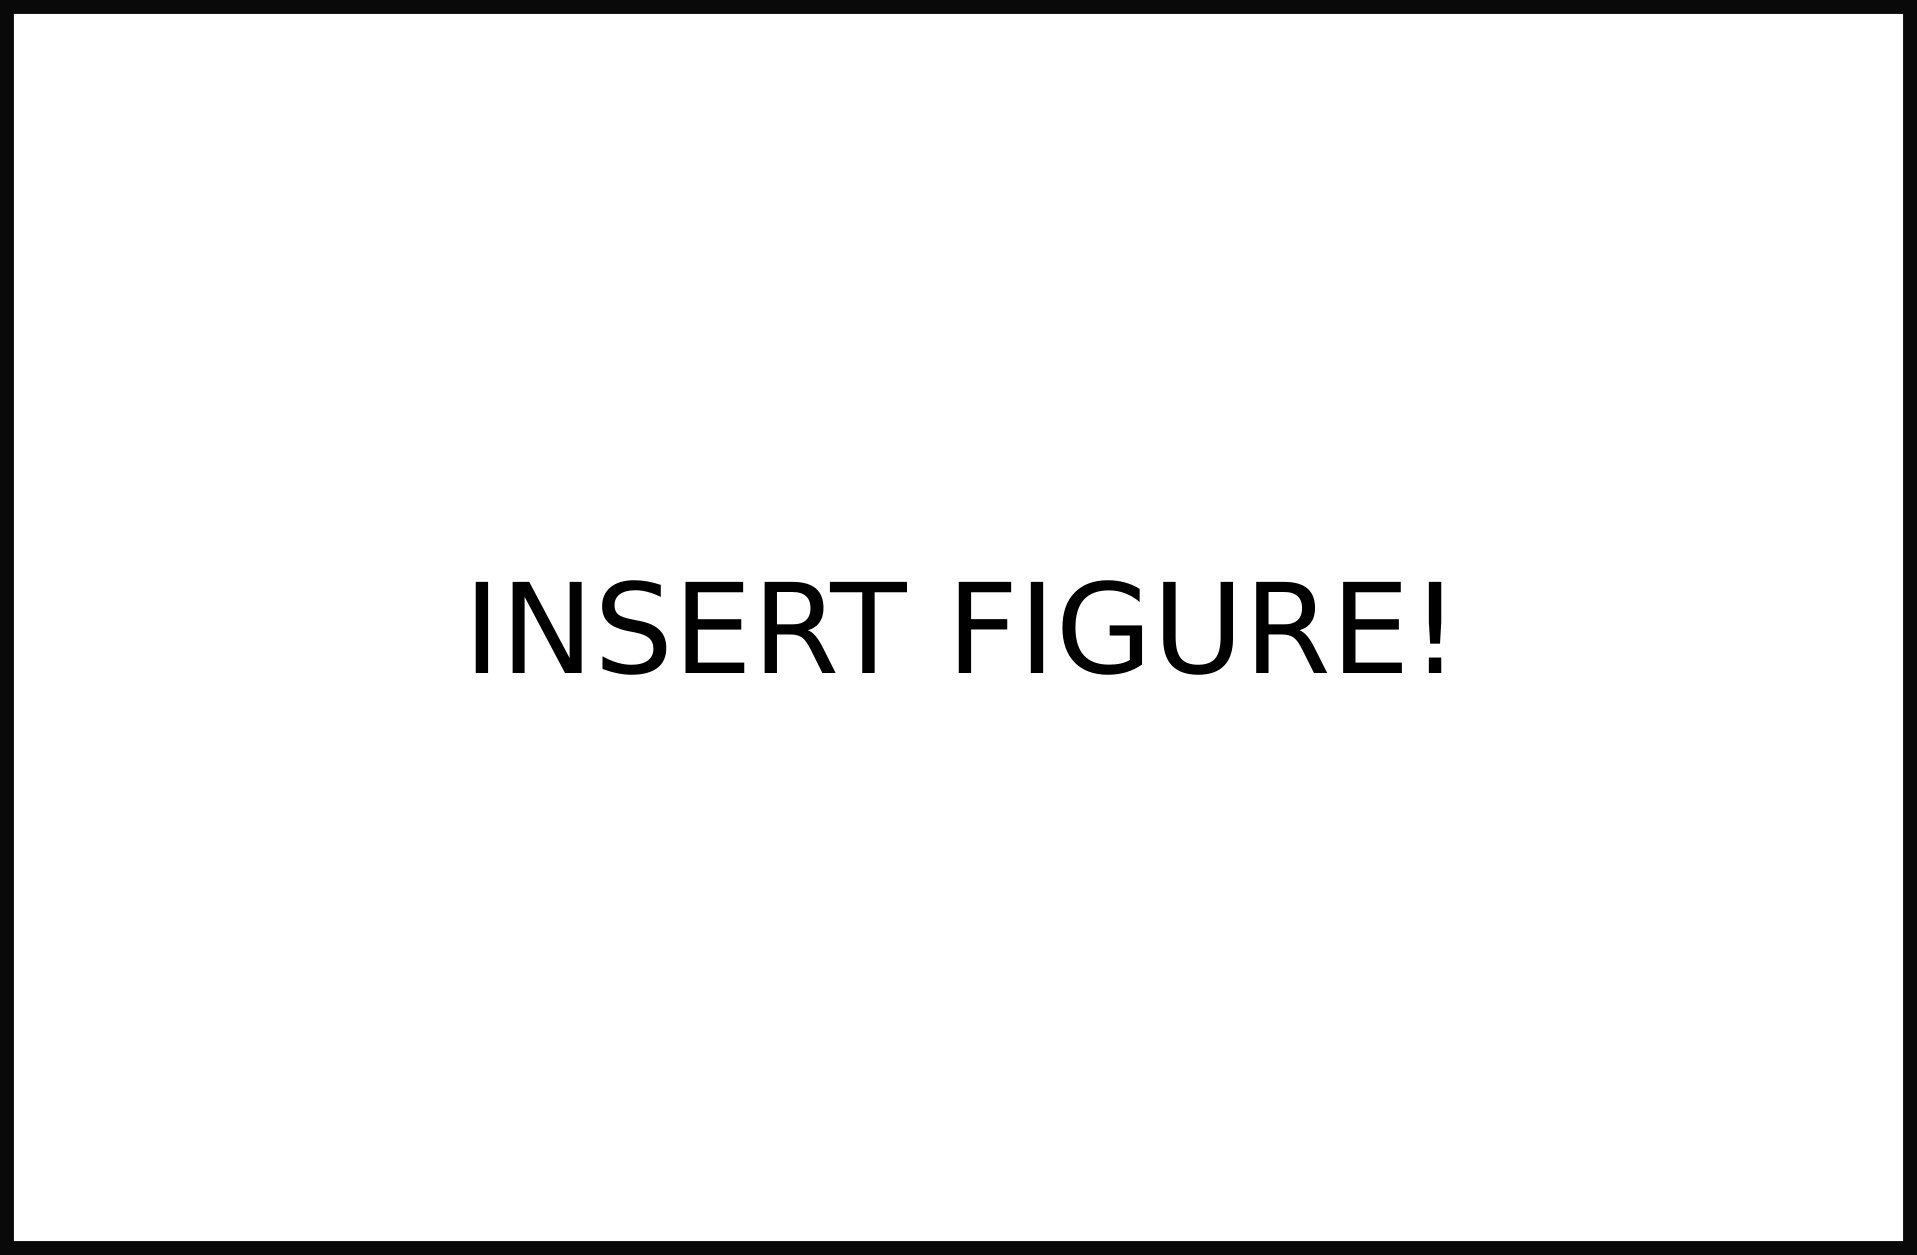
\includegraphics[width=0.8\textwidth]{img/insert_figure_here.png}
\caption[Multi-Robot Task Allocation Taxonomy]{\label{fig:mrta-taxonomies} \textit{Multi-Robot Task Allocation Taxonomy}. Description}
\end{figure}

\newpage

\section{Taxonomy of Routing Problems} \label{sec:vrp-taxonomy}

The following section deals with the \textit{vehicle routing problem (VRP)}. Specifically this entails the introduction of the origins of the vehicle routing problems, it's early development within the research community and it's relationship to other similar fields and topics. Thereafter more recent developments of the field are mentioned, specifically concerning the idea of \textit{synchronization}, due to it's relevance to this thesis and the connection towards MRTA. After that, some possible taxonomies for the field of VRP are showcased. The section ends with a comparison of MRTA and VRP taxonomies, which highlights the conceptual differences within the respective fields approaches.

\subsection{Variants of the vehicle routing problem}

% Here I want to introduce the vehicle routing problem.
% I definitely have to mention this one paper, which has created it and this is probably also the 
% correct section to mention, which kinds of other constraints there could be for a vehicle 
% routing proble aside from the ones I will mention later on.

% I guess I would start with something like "yeah so this was the first problem of its kind"
% and it stems from the TSP.
Although the exact origin of the VRP is unclear, the "Truck Dispatching Problem" by Dantzig and Ramser in 1959 \cite{dantzig_truck_1959} is often mentioned as one of the earliest publications to introduce the general idea of the vehicle routing problem.\\
The VRP is an optimization  problem which is related to the much more well known \textit{traveling salesman problem (TSP)}. The TSP can be described as follows: A set of spacially distributed cities is given and a traveling salesman has the intention to visit every city exactly once. The optimization objective is to find the route which includes all these cities and ends at the starting location, which minimizes the total travel distance between the cities. For a more detailed description of the TSP refer to Flood  \cite{flood_traveling-salesman_1956}. The VRP in turn is seen as an extension of the TSP. For the VRP there is also a set of locations which have to be visited. Additionally it is assumed that there is one "depot" location which contains a fleet of vehicles. These vehicles are available to visit the required locations. The problem is additionally constrained in such a way that every location is only to be visited once by any vehicle and every vehicle has to return to the depot after it's last job. The objective of this problem is also to minimize the cumulative travel distance of all vehicles. The mathematical model for the VRP represents the customer locations as nodes in a network graph, where the edges between these nodes represent the travel costs between locations. The problem is formulated as a \textit{mixed integer programming problem (MIP)}, where a series of constraints enforces the above mentioned properties of a valid solution. For an illustrative example of a VRP solution refer to to figure ?. \\
% FOOTNOTE: Clarify the naming conventions for the vrp are not absolutes
% Then I would go on to say that over the years it has become more popular especially with the 
% operations research communinty and the logistics industry. This has in turn created the more
% well known additions to the problem such as the time windows. 
For one thing, the VRP has been studied on a more theoretical basis as a mathematical optimization problem. (Do I want an example here? of an early theoretical paper for VRP) But it also had a very concrete practical implication: Due to it's structure, it served as a simplified model for physical distribution processes of the logistics industry. The vehicles would represent trucks and the locations would represent drop-off destinations for some goods. Subsequent improved solutions for the VRP would then go on and also improve planning for real life delivery problems. Examples for this could be seen by publications, which have applied the vehicle routing problem for newspaper distribution [?], milk truck routing [?] and SOME OTHER EXAMPLE [?] just to name a few. As the broader field delivery operations was the main application for the vehicle routing problem in the earlier years, the requirements of these very operations have had a big impact in the creation and investigation of new VRP variants.\\ \\
% This figure is supposed to contain a small illustration of how to imagine a VRP
% possibly also include ideas of time windows and capacities?
\begin{figure}
\centering
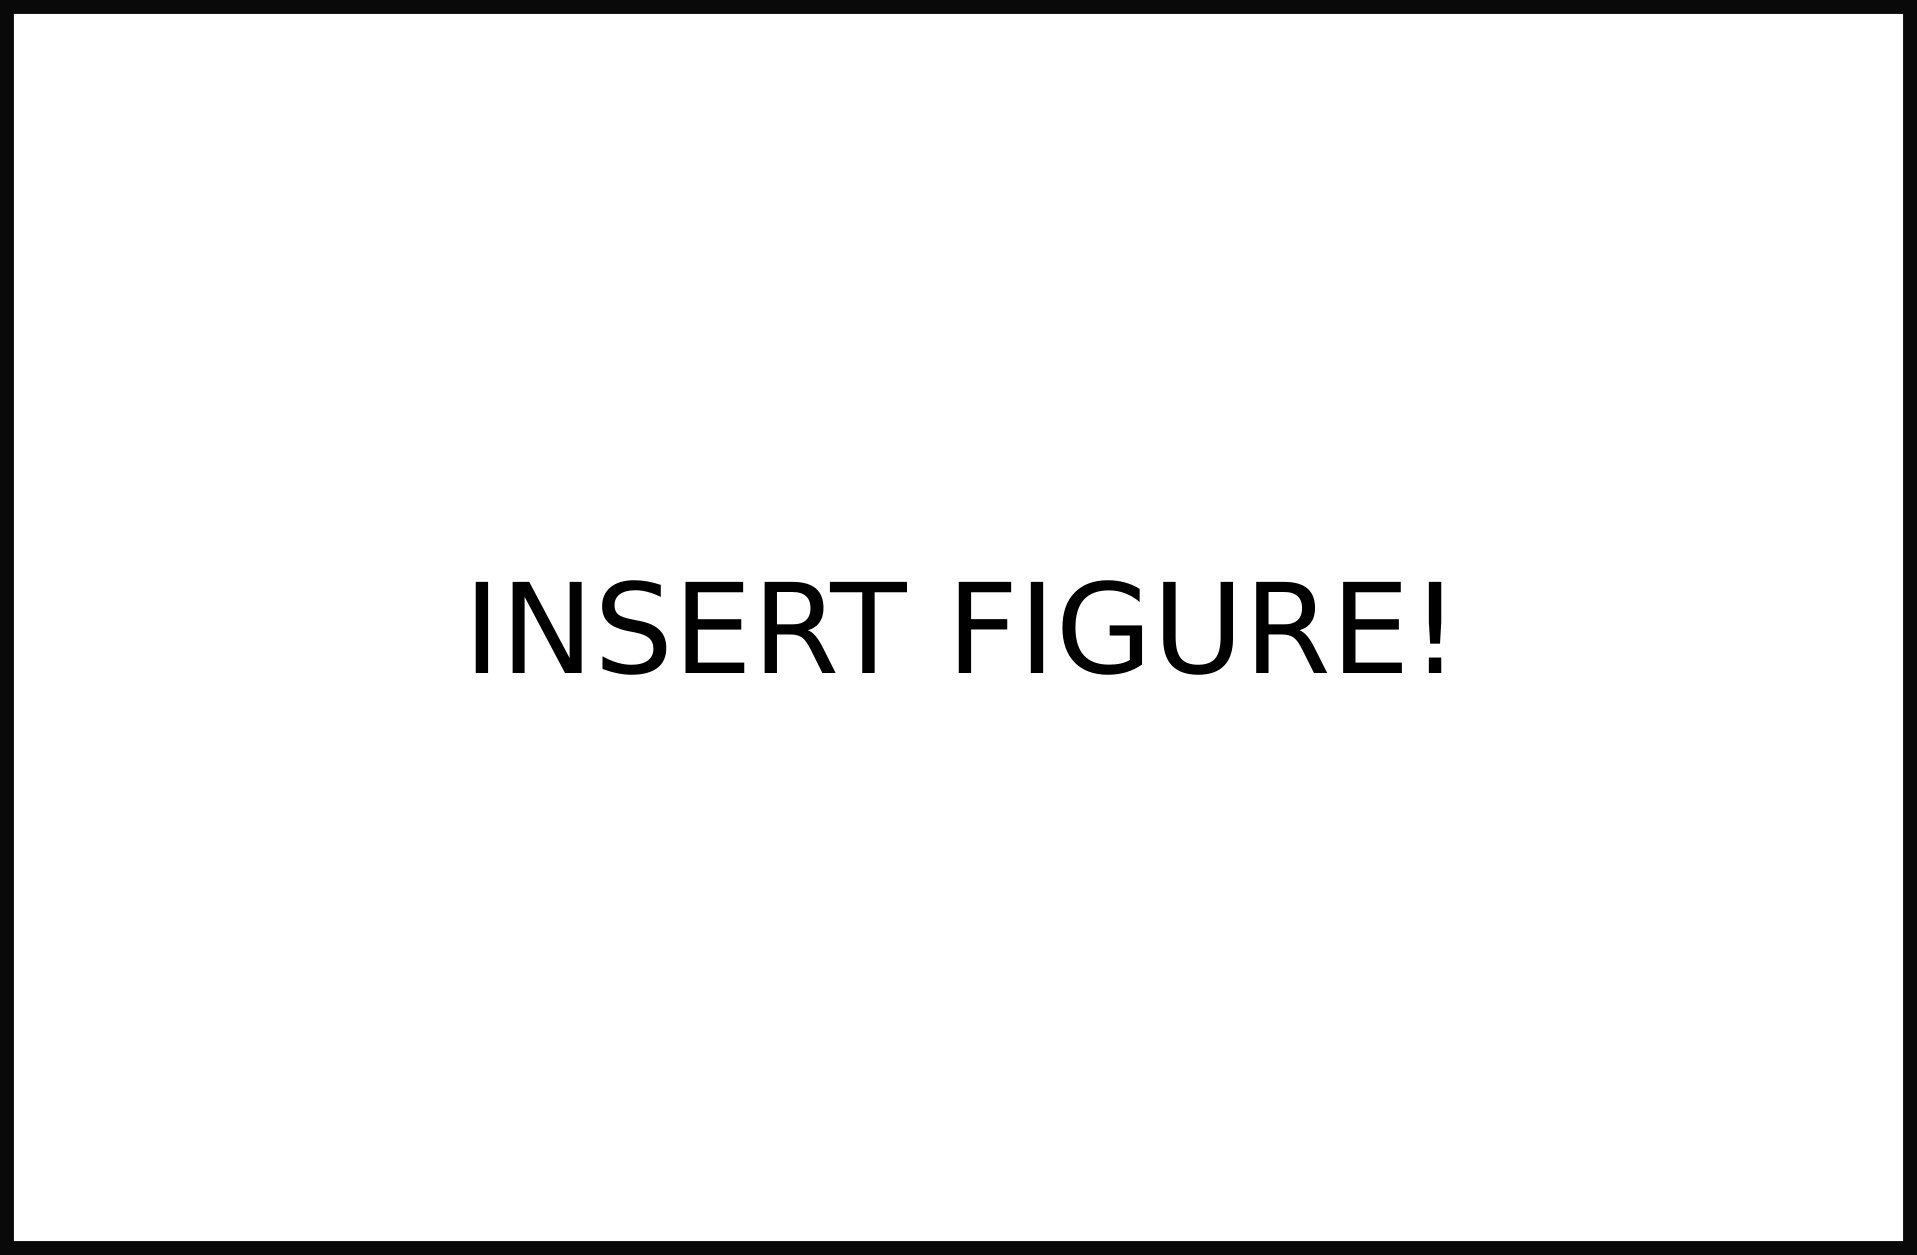
\includegraphics[width=0.8\textwidth]{img/insert_figure_here.png}
\caption[Multi-Robot Task Allocation Taxonomy]{\label{fig:vrp-illustration} \textit{Illustrative example of vehicle routing problem}. Description}
\end{figure}
% VRP WITH TIME WINDOWS
Arguably the most influential variant of VRP was the introduction of 'time windows'. This \textit{vehicle routing problem with time windows (VRPTW)} first off introduces a scheduling dimension to the previous routing problem. The start and end time of every visit and every vehicle are now being kept track off. This information is important because it is now also possible for a location to define a time window, where the starting time of a visit must lie in between a maximum and a minimum value. The practical importance of this addition is the fact, that in real life delivery applications customers often only have a limited availability. In his publication of 1984, Solomon \cite{solomon_algorithms_1987} presents a first in-depth analysis of time window aspect within vehicle routing. The author conducted a variety of computational experiments on  a set of generated problem instances using custom heuristics.\\
% CAPCITATED VEHICLE ROUTING PROBLEM
Another important addition to the VRP was the principle of vehicle capacity. Within the \textit{capacitated vehicle routing problem (CVRP)} each vehicles is also associated with a certain available capacity. The locations in turn also define a required capacity. For each vehicle the available capacity presents an upper limit towards the number or visits it is physically able to perform before having to return to the depot.\\
% HETEROGENEOUS VEHICLE ROUTING PROBLEM
% - Also cite other paper for the HVRP
% - Also mention the site dependent VRP as a specifc subtype !
An important variant for this thesis specifically is the \textit{heterogeneous vehicle routing problem (HVRP)}. This generic terminology has been used to describe many different variants of the VRP already. The commonality in those cases being the heterogeneity of one or more attributes of the vehicles or locations. Some common examples would be that different vehicles might have different properties such as travel speed or storage capacity. In some case visit durations are defined individually for different vehicles and sometimes visit locations are even exclusive to some specific vehicle type. Golden et al. \cite{golden_fleet_1984} for example introduced the "fleet size and mix" vehicle routing problem in 1984. This is a subcategory of the heterogeneous VRP, which considers varying vehicle capcities for different vehicle types. Additionally the problem captures the idea of a variable fleet size, which can be summerized as follows: "If there is an infinite pool of vehicles available and routing costs drop with the number of vehicles, but every additional vehicle introduces a static cost, which is the optimal number of vehicles to use?". The paper developed several heuristic algorithms as well as a lower bounding procedure to tackle the problem.\\
% DYNAMIC VEHICLE ROUTING PROBLEM
A variant, which has been getting more attention more recently is the \textit{dynamic vehicle routing problem}. For this it is necessary to understand the static and limited nature of the classic VRP: Let's say as an example a delivery company wants to employ the VRP as a model to optimize their routes for each work period. At the beginning of each day, a plan would be generated from the information about available vehicles, drop-off locations etc. Following the creation of the plan the vehicles would leave the depot to execute this plan. This means the application scenario would always be strictly divided into the planning phase and the execution phase. The dynamic VRP takes into account the fact, that in reality there are often unforeseen events or new information during the execution of a plan. It's basis is to investigate algorithms, which can modify plans following the revelation of new information about the system.
% In the most recent years the problem has also seen more attention from other industries and 
% and thus created more variations

\subsubsection{Arc-routing problems}

lol

\subsubsection{Problems with profits}

% BASIC IDEA BEHIND ROUTING PROBLEMS WITH PROFITS
The basic formulation of the vehicle routing problem such as given by \cite{dantzig_truck_1959} or \cite{golden_fleet_1984} only includes the minimization of the routing costs as well as the satisfaction of some capacity constraint. Additionally every customer node has to be visited. A related optimization problem is presented by the so called \textit{routing problems with profits}. These kinds of problems introduce two changes to the VRP concept:
\begin{enumerate}
\item Only a subset of nodes can be visited.
\item Every node is additionally associated with a \textit{profit}.
\end{enumerate}
The optimization objective thus also includes the dimension of choosing the most suitable nodes. These chosen nodes have to fit both in terms of provided profit as well as expected travel cost. The \textit{profitable tour problem (PTP)}, \textit{price collecting traveling salesperson problem (PCTSP)} and the \textit{orienteering problem (OP)} are some examples for this problem class. The major difference between them being whether the profit or the cost is implemented in the objective function or a constraint of the problem formulation. \cite{vansteenwegen_orienteering_2019}\\ \\
% ORIENTEERING PROBLEM - Do I find sources for all of these.
From the above mentioned problems, the orienteering problem is the most well known. The problem's name originated from the sports game of 'orienteering' (SOURCE?), where a player has to visit certain checkpoints and return to the starting location within given time frame to score points. At it's core the base OP is more similiar to the traveling salesman problem, because it only considers one vehicle. The objective is to maximize the profits, while there is an upper limit to the travel costs enforces by an additional constraint.\\
Like the VRP, the OP has spawned various variations and extensions over the years. The most commonly used extension, the \textit{team orienteering problem (TOP)} considers a fleet of vehicles to be available. Other extensions include time windows [?], time depenent travel times and or profits as well as \\ \\
For a detailed introduction to routing problems with profits refer to \cite{vansteenwegen_orienteering_2019} and for a survey of the literature see \cite{vansteenwegen_orienteering_2011}.
% The OP with stochastic profits is discussed in more detail in Ilhan et al. (2008).

\subsection{Synchronization in Vehicle Routing}\label{sec:vrp-syn}

% I guess at first I would be kind of introduce what synchronization is (very shortly).
% Other things I have to mention:
% - The survey of synchronized problems
% - The important individual papers
% - Which other fields contribute to this idea of synchronization
% - Castillo PhD
% The question is in which order I will be mentioning these points? 
Bredström and Rönnqvist (2008) \cite{bredstrom_combined_2008} propose a model for the "combined vehicle routing and scheduling problem with temporal precedence and synchronization contraints". The model is a generalization of the vehicle routing problem with time windows. In this work the term synchronization is used synonymously for a cooperation between two vehicles. A cooperation requires the vehicles to visit a node at the same time to complete the task. The authors illustrate the requirement of synchronization constraints with examples from homecare staff scheduling, forest operations and airline scheduling applications.\\
Rasmussen et al. (2010) \cite{rasmussen_home_2012} applies a model with synchronization constraints to the \textit{home health care problem (HHCP)}. For the field of home health care temporal and ordering constraints are important for several reasons: Cooperation between two mobile nurses is required during the bathing of disabled patients for example and precedences are enforced by the strict timing requirements between the admission of specific drugs. The work also introduces the precedence formulation, which includes a minimum and maximum time frame definition between two ordered tasks. This allows for the definition of 5 different temporal relationships between two tasks. For a detailed description refer to section \ref{lol}.\\
For an overview of the home health care problem in general, refer to the recent work of Fikar and Hirsch \cite{fikar_home_2017}. The authors review single and multi period routing problems in the context of home health care. Different common objectives, constraints and solution methods are showcased for both variants.\\
% How in depth could I describe this system for synchronization here?
While the home health care problem is a major source of advancement for routing problems with synchronization constraints there are other related fields as well: The technician and task scheduling problem \cite{cordeau_scheduling_2010}, also called technician routing and scheduling problem (TRSP) \cite{pillac_technician_2011} is generally concerned with the routing/scheduling of teams of service technicians to a set of customer locations. Synchronization can sometimes be observed as direct cross dependencies between tasks, but is more often realized in the form of \textit{teaming}. Teaming refers to the grouping of individual technicians (vehicles) for certain tasks based on the consideration of their individual properties.\\
In his PhD, Castillo-Salazar \cite{castillo_salazar_optimisation_2015} coins the term of the \textit{workforce scheduling and routing problem (WSRP)} which attempts to provide a generalized model for previously mentioned problems of personnel routing and scheduling such as the HHCP and TRSP. Among time window, synchronization and precedence constraints the WRSP also includes more domain specific constraints such as break and overtime regulations, transport modality and employee preferences.\\
% Wie viel von der PhD soll ich hier noch erwähnen?
Drexl \cite{drexl_synchronization_2012} provides an extensive literature survey of vehicle routing problems with synchronization constraints. Based on the existing literature, five categories of general synchronization types are identified. The term 'synchronization' in vehicle routing refers to some sort of coupling between the vehicles. The following types of synchronization present different aspects of where this coupling is introduced to the problem:
\begin{itemize}
\item \textbf{Task synchronization} This refers to the very basic idea that in vehicle routing there is almost always more than one vehicle. Together with the constraints, that every node is only to be visited once, this of course introduces such a coupling. If a node is already visited by a vehicle, it automatically cannot be visited anymore by any other vehicle. Thus almost all vehicle routing problems contain some form of synchronization in regards to the task distribution among the available vehicles.
\item \textbf{Operation synchronization} For some problems it is the case, that operations have some form of dependency between each other. An example would be the administration of several drugs for one patient in the HHCP. The drugs need to be administered in tight time intervals. This means, that depending on the scheduling of the first task of such a dependency, the second one is imposed with a dynamic time window. In that way, operation synchronization refers to the type of temporal synchronization discussed previously.
\item \textbf{Movement synchronization} To illustrate this, consider the example of the vehicle routing problem with trailers and transshipments (VRPTT) \cite{drexel_phd?}. This problem consists of active vehicles (trucks) and passive vehicles (trailers). A trailer is needed to perform the delivery, but has to be coupled with a truck to actually move. As such the movement of one type of vehicle has to be synchronized with another compatible vehicle. The benefit of this example in particular is that trailers could also be decoupled and positioned at empty parking lots for other trucks to pick up. This introduces a lot more realism (but also complexity) to the problem.
\item \textbf{Load synchronization} In most vehicle routing problems the concept of capacity defines how many nodes can be visited by a certain vehicle, before having to return to the depot. Now with load synchronization there could be the possibility of transferring a partial amount of one vehicles capacity to another one.
\item \textbf{Ressource Synchronization} This type of synchronization is relevant when different vehicles compete over a common, scarce ressource. This is something, which can be observed with many MRTA problems, which make the assumption of 'limited communication'. In such a case the small communication bandwidth with a central processing unit for example would be such a common resource. This would also present some form of coupling, in which vehicles ability to communicate would be tied to all the other vehicles as well.
\end{itemize}

\subsection{VRP Taxonomies}\label{sec:vrp-taxonomies}

% BODIN AND GOLDEN. FIRST TAXONOMY WHICH IS REALLY USEFUL
Bodin and Golden (1981) \cite{bodin_classification_1981} present a taxonomy for vehicle routing and scheduling problems. The problem classification taxonomy includes a total of 13  categories. These categories cover a number of different attributes such as the nature of capacity constraints, the underlying network graph, vehicle heterogeneity and the objective function among other things. A particular emphasis is made towards the nature of temporal constraints. Three cases are identified for the different variations of available time frames to complete a task:
\begin{itemize}
\item The time of arrival is fixed in advance. The problem thus boils down to a pure \textit{vehicle scheduling problem (VSP)}, as the only objective is to meet the tight timing constraints.
\item Tasks define time windows of availability. The problem is classified as a \textit{combined vehicle routing and scheduling problem (VRSP)}.
\item No timing constraints are imposed by the tasks. The problem is classified as a pure \textit{vehicle routing problem (VRP)}
\end{itemize}
This differentiation implies, that VRSP would be the correct naming convention for every problem which includes some type of temporal aspect. Although this is sometimes the case, it is not used consistently throughout the literature. More often the term VRP is used to describe all kinds of variations including those with temporal constraints.\\
Bodin and Golden also introduce a basic classification for solution approaches, where they have identified 7 rough categories. These emphasize the different heuristic strategies, which have been used primarily at that time.\\ \\
% CLASSIFICATION LANGUAGE BY DESROCHERS
Desrochers et al. (1990) \cite{desrochers_classification_1990} developes a classification scheme for the VRP, which shares some common characteristics with \cite{bodin_classification_1981}, but also significantly extends the scope. Notable extensions include the possibility of multi depot and multi time window definitions, as well as synchronizations constraints. In addition to those extensions, a custom definition language is developed to accurately describe a certain configuration of those properties. Building on this definition language Desrochers et al. (1999) \cite{desrochers_towards_1999} introduces a "model and algorithm management system for vehicle routing and scheduling problems". This system aims to support the modeling process of physical distribution processes, as well as the selection and implementation of solution algorithms. Given a certain configuration of problem parameters, the implementation of this decision support system provides a list of well known VRP related problems ranked by their degree of similarity. This information about the similar mathematical models and their solution approaches guides the process of implementing solution schemes for a custom problem variation.\\ \\
% THE TAXONOMIC REVIEW ABOU THE PAPERS
% I think I have to change this and maybe explain it a little bit more in detail?
Eksioglu et al. (2009) \cite{eksioglu_vehicle_2009} conducts an exhaustive study of the existing VRP literature. The resulting taxonomy is based on Bodin and Goldens initial proposal, but greatly extends the scope and detail of both previously mentioned attempts. The taxonomy consists of five major categories, totaling 26 evaluation criteria:
\begin{itemize}
\item \textbf{Type of study} refers to the type of publication. Types may differ as much as a purely computational study or a theoretical proof.
\item \textbf{Scenario characteristics} includes all those characteristics, that are not a part of the constraints embedded into the solution, but part of the problem scenario.
\item \textbf{Problem Physical Characteristics} summerizes the factors which directly affect the solution.
\item \textbf{Information Characteristics} deals with the nature, accessibility and processing of the information about the problem. This may range between variations of static, dynamic and stochastic properties.
\item \textbf{Data Characteristics} is used to classify whether or not data has been used in the context of a computational study, for example. It also addresses the origin of this data, which may be based on real world problems or computationally generated.
\end{itemize}
The approach differs from previous attempts by creating an evaluation scheme geared towards the VRP literature instead of just the problems. This can be seen with the categories 'type of study' and 'data characteristics', which are properties related to the publication from which a problem has originated from and not the problem itself.\\
A notable addition in respect to the previously mentioned approaches is the inclusion of 'information characteristics' and thus the possibility of describing (partially) dynamic vehicle routing problems. However, the authors note about their own effort: "The current attempt to define a taxonomy for the VRP literature may have its own disadvantages but it does not suffer from ambiguity [...]. In fact, this taxonomy may be too detailed." \cite[p.1477]{eksioglu_vehicle_2009}\\ \\
% RICH VEHICLE ROUTING TAXONOMY
Lahyani et al. (2015) \cite{lahyani_rich_2015} presents a taxonomy consisting of two major categories and a total of 16 evaluation criteria. The major categories are called 'scenario characteristics' and 'problem physical characteristics' much like in Eksioglu et al., although the actual subcategories d´iffer. This taxonomy also focuses on the specific problems rather than on the more general literature. It can be seen as an effort to reduce the complexity presented in the previous approach. Considerations of information characteristics are still maintained, albeit condensed into less, more generalized criteria.
% Maybe mention that eksioglu is very broad.

\subsection{Comparing MRTA and VRP taxonomies}\label{sec:problem-comparison}

% SHORT INTRODUCTION
The fields of multi robot task allocation and vehicle routing share various commonalities. At their core they are both mathematical optimization problems, which aim to create routes/schedules for a team of (mobile) agents to optimize some kind of cost or profit function. Despite their inherently similiar structure, they also have some notable differences. These differences also reflect in the respective field's approach to creating taxonomies. The following comparison is supposed to highlight those differences between the previously mentioned taxonomies of both fields, but also outline how some categories can still be related to one another. \\ \\
% DIFFERENT STRUCTURES
The most notable difference is in the granularity and generalization displayed within the taxonomies. The MRTA approach represented by Korsah et al. \cite{korsah_comprehensive_2013} focuses on a small amount of generalized categories thus resulting in a small amount of 21 possible combinations. The VRP approaches on the contrary have a lot of categories for very nuanced details of a problem, which in turn have multiple possible classification values. This goes as far as Eksioglu et al. having 26 evaluation criteria alone, each having around 2-6 possible values, resulting in a huge number of possible combinations. This is due to the fact that different application scenarios for physical distribution processes have introduced very specific constraints and variations over the years. The term VRP has been used to unite a lot of different ideas in the past and is thus arguably an inherently more generic term than MRTA.\\
% EXPLAIN THE RELATIONSHIP WITH THE VENN DIAGRAM
In general the relationship between the two fields can be visualized by a venn diagram alike figure \ref{fig:venn-vrp-mrta}. Both fields have their own quirks, which are mostly exclusive to themselves, but also overlap in certain areas. As such Korsah's taxonomy lists several VRP publications as examples of it's categories and VRP models/algorithms are applied to robot routing and scheduling problems.
\begin{figure}
\centering
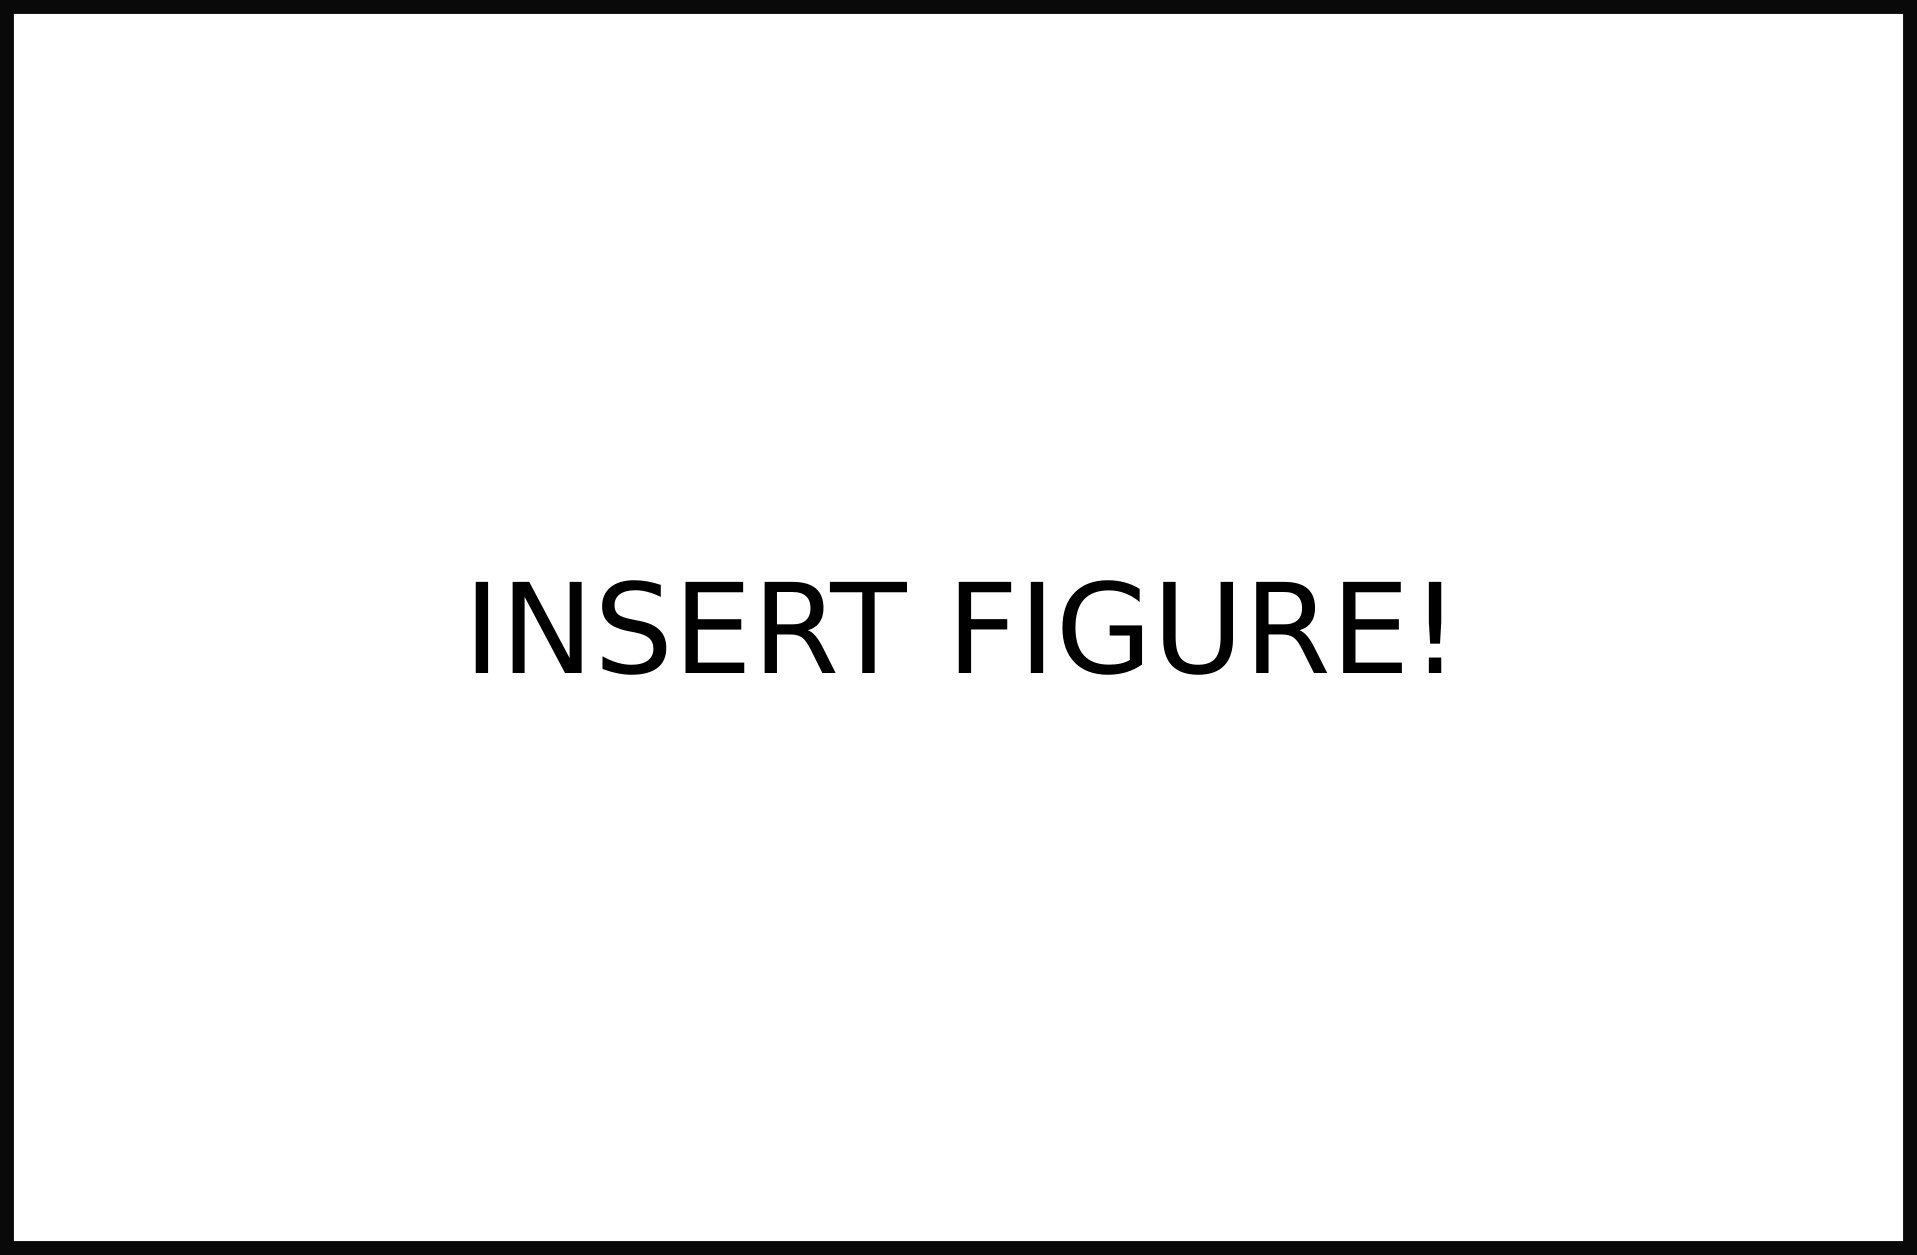
\includegraphics[width=0.8\textwidth]{img/insert_figure_here.png}
\caption[Multi-Robot Task Allocation Taxonomy]{\label{fig:venn-vrp-mrta} \textit{Relationship between MRTA and VRP}. Venn diagram visualizing the relationship between the fields of multi robot task allocation (MRTA) and vehicle routing (VRP)}
\end{figure}
A notable similiarity can be observed with the respective fields emphasis on temporal and synchronization constraints, as it is apparant with Nunes' MRTA/TOC taxonomy \cite{nunes_taxonomy_2017} and the recent increased effort towards vehicle routing problems with synchronization constraints (sec.\ref{sec:vrp-syn}).\\
Additionally many idea from the respective fields can be put into relation with each other illustrated by the following examples:
\begin{itemize}
\item The fact that agents can start at any location in a MRTA scenario can be seen a multi depot VRP.
\item The idea of time-extended assignment of MRTA tasks describes the fact, that knowledge about the nature of tasks is known from the start, therefore this directly relates the to scenario of a static VRP. Instantaneous assignment on the other hand implies, that knowledge of tasks will be released only during the execution period. This can be roughly translated to the dynamic VRP, where additional knowledge may also inluence the system during execution.
\item ...
\end{itemize}

\newpage

\section{Approaches for solving vehicle routing problems}\label{sec:vrp-approaches}

This section provides a short overview over the algorithms and approaches applies to solving various vehicle routing problems. Throughout the literature it became apparent, that there are mainly two fundamental approaches being used nowadays: \textit{Metaheuristics} and \textit{Exact methods}. The sections \ref{sec:metaheuristics} and \ref{sec:exact} will deal with those respectively. Another interesting development is within the field of interactive optimization methods. These approaches aim to include a human aspect into the planning process, hoping to utilize the human intuition for such problems. Only a brief introduction of this field is presented in section \ref{sec:interactive}, as a complete consideration is outside if this thesis' scope. The section will conclude with section \ref{sec:others}, which will refer to some other exotic methods sometimes encountered in literature.

\subsection{Metaheuristics}\label{sec:metaheuristics}

% SMALL MOTIVATION AND DEFINITION FOR METAHEURISTICS IN GENERAL
In the early days of VRP research, the most prominent solution methods were so called heuristics. This term simply referred to a solution methodology, which just 'made sense' for human understanding. These methods were not strictly based on some mathematical or theoretical property of the problem. Instead they presented decent solution strategies created mostly from human intuition. These heuristics were furthermore strategies, which were tailored very precisely to a specific problem formulation. This approach had the obvious disadvantage, that for every new problem or slight change in the basic formulation sometimes an entirely new heuristic had to be created.\\
The term metaheuristic refers rather to more generic solution schemes, than specific algorithmic implementations. The idea is to find a generally applicable method, which only has to be slightly adapted to be used for different problem types. Because of their decent performance, low computational costs and flexibility metaheuristics have become the most prominent solution in many optimization related fields, including vehicle routing problems.\\ \\
% NOW ACTUALLY STARTING WITH THE TAXONOMIC STRUCTURE OF THE THING
Elshear and Awad \cite{elshaer_taxonomic_2020} present a "taxonomic review of metaheuristic algorithms for solving the vehicle routing problem and it's variants". In their work they review about 300 publications from VRP literature to create a classification scheme for the used metaheuristic approaches. A modified [A FOOTNOTE WOULD BE NICE] version of this scheme can be seen in figure \ref{fig:metaheuristics}. The approaches are roughly divided into the two categories of 'single solution based' and 'population based' metaheuristics. Thereby the population based ones can be further divided into 'evolutionary computation' and 'swarm intelligence'. Roughly speaking, the single solution based methods work by iteratively improving a single solution and the population based ones maintain a set of different solutions. Population based methods then seek to advance this whole population of solutions by means of selection, comparison, modification and others. Evolutionary computation generally lends conceptual strategies from the biological principle of evolution. Swarm intelligence methods are often inspired by behavioural patterns of swarm-based animals, but also includes other, less intuitive approaches.\\
Elshear and Awad additionally evaluated the popularity of each approach by relative frequency of occurrence within the literature. Their results show that for single solution based methods 'tabu search' is the most popular with 30.1\% followed by variable neighborhood search (22.8\%), large neighborhood search (15.4\%) and simulated annealing (12.2\%). For genetic computation, the genetic algorithm is clearly the most popular with 57.5\%, followed by it's close relative the memetic algorithm (16.25\%). For swarm intelligence methods 'ant colony optimization' (46.7\%) and 'particle swarm optimization' (30\%).\\ \\
% FIGURE WHICH SORT OF ILLUSTRATES THE STRUCTURE OF THESE
\begin{figure}
\centering
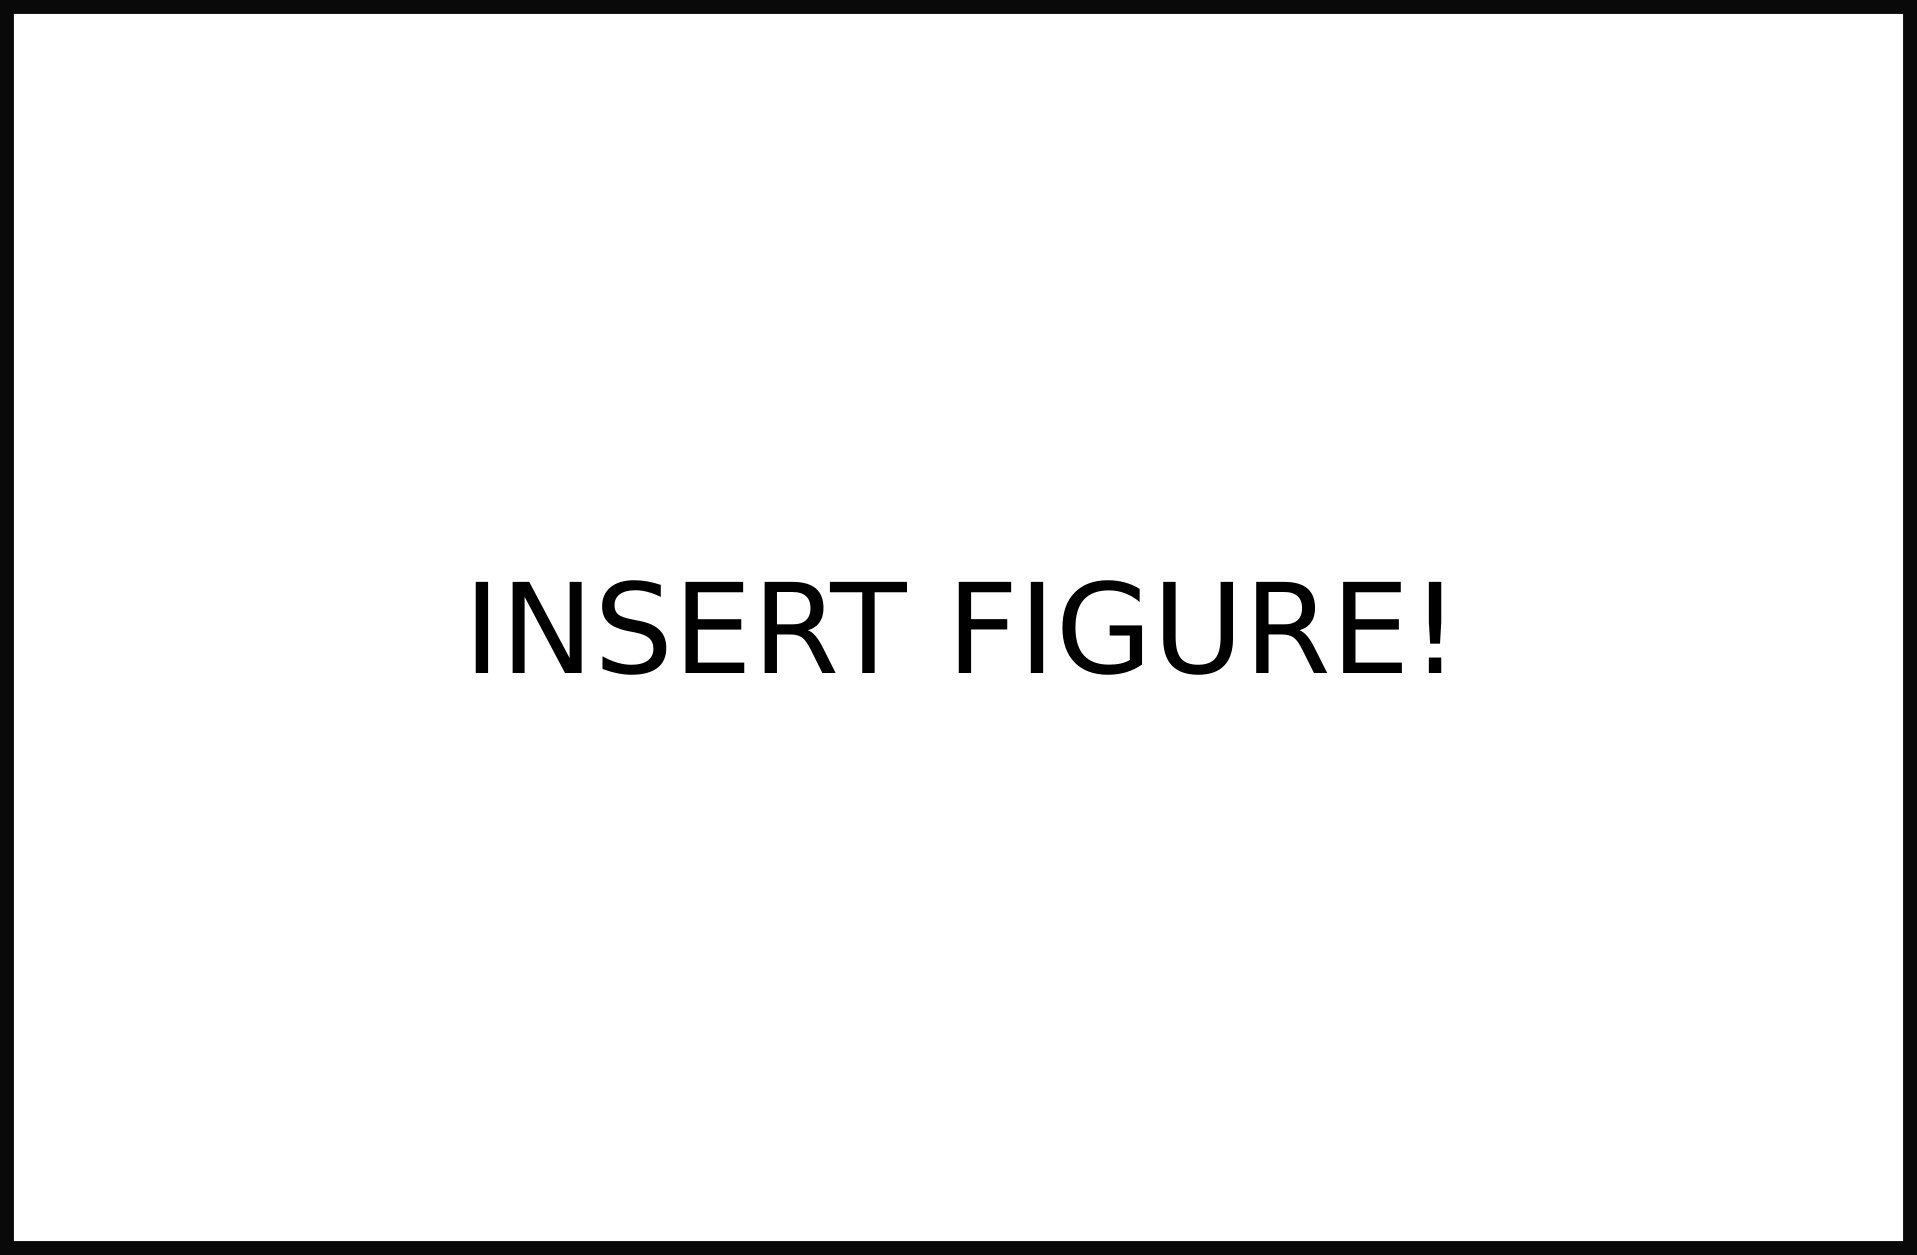
\includegraphics[width=0.8\textwidth]{img/insert_figure_here.png}
\caption[Structure of metaheuristic methods]{\label{fig:metaheuristics} \textit{Classification structure of metaheuristic methods}. I do need to say that is was based on the paper but changed.}
\end{figure}
% NOW ALSO MENTION WHICH OTHER GENERAL OVERVIEWS THERE ARE
Gendreau et al. \cite{gendreau_metaheuristics_2008} additionally provides a categorized bibliography for only the most common metaheuristics. Additionally they only consider the solution of the base VRP.\\
Vidal et al. \cite{vidal_heuristics_2013} presents a more recent literature survey, which specifically considers the different variations of the VRP. Aside from metaheuristics, their work also considers classic heuristic approaches.\\ 
For a detailed introduction to the topic of (meta-)heuristic algorithms, \cite{marti_handbook_2018} and \cite{gendreau_handbook_2019} provide a good introduction and starting point for further exploration. The books contain formal as well as practical information for many types of different heuristic and metaheuristic approaches, which were mentioned in this section.\\ \\
The following subsections will provide a brief, high-level explanation of the most common algorithms for the different types of metaheuristics, as well as some example publications related to the VRP.
% MENTION HANDBOOK OF META HEURISTICS´

\subsubsection{Single solution based}

% TABU SEARCH
At it's core the tabu search (TS) algorithm is a local search procedure. This means, that small changes are made to a 'current solution'. These small changes can be interpreted as local search move, respective to some search operator. These modified solutions are evaluated regarding their cost/objective value. Usually the solution with the best improvement out of those would be chosen as the next 'current solution'. The TS algorithm however also allows the acceptance of solutions, which worsen the solution. This is a means to escape bad local optima. Additionally, TS introduces a short term memory which stores recently evaluated solutions. These solutions are blocked for some time to avoid short-term cycling.\\
Cordeau and Laporte \cite{cordeau_tabu_2001} implement a tabu search approach for the SDVRP with time windows. They conclude that the TS is an efficient approach for their generated data set.\\
Nguyen et al. \cite{nguyen_tabu_2013} create a TS algorithm for the time dependent multi-trip vehicle routing problem with time windows. With some additional extensions to the procedure they clearly show improved performance towards contemporary literature.\\ \\
% SIMULATED ANNEALING
The simulated annealing (SA) algorithm is inspired by the physical process of 'annealing' used in metallurgy. Annealing refers to an intentionally slowed/controlled cooling process of molten materials, also used for the production of glass for example. The slow change in temperature helps the individual atoms to reposition themselves properly, which avoids static tension in solid state. The idea behind simulated annealing is to introduce a controlled temperature curve to the optimization process. High temperatures increase the possibility that bad results of a local search are accepted by the algorithm. This implies that for low temperatures mostly only improved solutions are accepted. Ideally, the algorithm would thus explore the search space more thoroughly in the beginning and focus on convergence only later on.\\
Afifi et al. \cite{afifi_simulated_2013} proposed a simulated annealing algorithm for the vehicle routing problem with time windows and synchronization constraints. The algorithm is partly compared with a commercial MIP solver and extended with a constructive heuristic.\\ \\ % DO I FIND MORE?
% VARIABLE NEIGHBORHOOD SEARCH
% - explain what a neighborhood is
Variable neighborhood search (VNS) is also a technique which uses local search moves. These local search moves are executed in terms of a specific search operator. In this context, the search operator is called a 'neighborhood'. The idea behind VNS is to define multiple of these neighborhoods. During the execution different operators are used iteratively. This is also a means of escaping local optima, which is based on the assumption that a local optima in the search space of one neighborhood is often not local optima in regards to some other neighborhood. Traditionally, the order in which the neighborhoods are applied is static. This order is usually based on some preliminary experiments and goes from the neighborhood which causes the greatest improvement to the objective value to the one with the least improvement.\\
Frifita et al. \cite{frifita_general_2017} propose a general variable neighborhood search procedure for the HHCP with time windows and synchronized visits. They find satisfactory performance on an exemplary data set.\\ 
Mankowska et al. \cite{mankowska_home_2014} implement an adaptive variable neighborhood search for the synchronized HHCP as well. The idea behind an adaptive version is to divide the optimization in two phases. The first phase will briefly figure out the optimal order of neighborhoods on each new problem instance dynamically. The second phase executes the standard VRP routine with this order.\\ \\
% LARGE NEIGHBORHOOD SEARCH
As the name of the large neighborhood search (LNS) algorithm suggests, it's main feature is the usage of large neighborhoods. This refers to the fact, that in every local search move a relatively big amount of variables is being changed. This approach stems from the observation, that these large neighborhoods usually lead to the discovery of good local optima. The way this is achieved in the LNS algorithm is by using a set of destroy and repair operators. The destroy operators define an algorithm to break the solution in some way, while the repair operators define heuristic algorithms to fix such broken solutions. A neighborhood is then defined as all those possible solutions, which can be achieved of subsequently applying a pair of destroy and repair operators. This way a lot of different neighborhoods can be achieved by exploring all possible combinations of operators. For the LNS, changing the neighborhood is also used as a means of escaping local optima.\\
Hojabri et al. \cite{hojabri_large_2018} present a large neighborhood search heuristic for the vehicle routing problem with time windows and synchronized visits. Constraint programming is additionally used a s a means of reconstructing broken solutions. The approach provided promising results for VRPTW literature benchmarks.\\
Liu et al. \cite{liu_adaptive_2019} implement an adaptive large neighborhood search for the VRPTW with synchronized visits. Their method is evaluated on literature benchmarks, outperforming most contemporary methods and even finding new best-known solutions.


\subsubsection{Population based}

% GENETIC ALGORITHM
% This part should maybe be a little bit longer, because I have focused on it.
The genetic algorithm (GA) is one of the approaches from the broader strategy of evolutionary computing. Many of these algorithms share a lot of similarities, because they are all based to some extent on the idea of biological evolution.\\ % Example of other thingys?
The genetic algorithms works by first generating a population of initial solutions. These initial solutions are usually created by some random procedure. This population is then iteratively subjected to the evolutionary cycle: The fittest individuals of the population in regard to their objective value are selected, these are then allowed to crossover to create a offspring population and finally a random mutation is applied to some members of this offspring with a certain chance. Applying the genetic algorithm to different kinds of optimization problems, poses the challenge of creating a suitable representation for a possible solution of the problem. This basic, stripped down representation is usually called the 'genotype'.Typical genotype representations are binary strings or lists, were each element encodes some property of a solution. Using these representations, appropriate crossover and mutation operators then have to be designed. These operators need to mix and modify the genotype representations in a meaningful way. A decoder function then maps these basic genotype representations of solutions to their actual phenotypic properties, such as the objective value.\\
Enterzari and Mahootchi \cite{entezari_developing_2020} create a genetic algorithm for modified home health care problem with synchronization constraints. They compare the performance of their algorithm with the optimal solutions obtained by a commercial solver. Near same results are achieved on those instance which were small enough to be solvable be the commercial solver.\\ \\
% ANT COLONY OPTIMIZATION
Ant colony optimization (ACO) is another nature inspired population-based metaheuristic. The inspiration stems from the cooperation mechanisms observed on real ant colonies, that allow them to find the shortest transportation path between a food source and their nest. At first, ants on the search for food would wander more or less randomly into the wild. On their way they would lay down a communication medium, called a 'pheromone'. When a next and would find such a pheromone trail, there would be some chance that it would follow it, depending on the strength of the trail. If it decided to follow, it would strengthen the trail even more with it's own pheromone. Naturally, the pheromone would thus accumulate on the shortest paths more quickly. This analogy is obviously the strongest for shortest path problems, but can be applied to any optimization problem as an abstract concept. For the algorithm, a number of artificial ants construct their own solutions. In each cycle, they choose the next element to add to their own partial solution from a set of common elements. If solutions evaluate to a good objective value, the elements involved in it get applied with a certain amount of pheromone. The amount of pheromone then in turn influences the selection of an element for the next construction process.\\
% Examples for aco?
Pereira et al. \cite{pereira_multiperiod_2020} implements an ACO algorithm for the multiperiod workforce scheduling and routing problem. The results show that it produces low gaps compared to the optimal solutions of a commercial solver, while needing drastically less computational time.

\subsubsection{Hybrid metaheuristics}

% INTRODUCTION WITH INTENSIFICATION VS. DIVERSIFICATION
% Do I find a reference for this?
When it comes to any metaheuristics, there are two important concepts involved in the consideration of every approach: \textit{Intensification} and \textit{diversification}. Intensification roughly refers to the ability of an algorithm to quickly converge to a better solution. Needing less iterations to achieve bigger objective value improvements obviously is a desirable property of any optimization process. If an algorithm always only accepted the best possible improvement, it would quickly get stuck in a local optimum though. Diversification now refers to the ability to escape these local optima. This is way almost all metaheuristics include the chance to accept a worse solution under some conditions. These two properties of intensification and diversification are contradictory to some extent and the design of a good heuristic optimization procedure relies on an appropriate balance between them.\\ % REFERENCE
Single solution based metaheuristics or local search procedures are said to be especially good at intensification, since they focus their effort on the incremental improvement of a single solution. Population based methods on the other hand are said to be good at diversification, due to the inherent diversity of maintaining a population of different solutions.\\ \\
% Maybe I ll find a paper, which directly has this as a topic
% HYBRID METAHEURISTICS
% I guess these claims would probably need a reference
The term \textit{hybrid metaheuristic} describes the combination of multiple different metaheuristic approaches, as they were discussed in the previous section. A lot of times this consists of the combination of one single solution and one population based method to combine their respective strengths of intensification and diversification. \cite{vidal_heuristics_2013}\\
Although, there are multiple ways of possible combinations: Two approaches of the same class could also be combined because of some other desirable features, there could be the combination of more than two methods and even just the integration of some other concepts concepts could be seen as a hybrid approach. An example of the last case would be the integration of some sort of short term solution cache, inspired by the tabu search algorithm. In general 'hybrid metaheuristic' refers less to a specific class of approaches, but hybridization is becoming more of an essential concept for the design of more sophisticated metaheuristics.\\ \\
The memetic algorithm (MA) can be seen as such a hybrid approach as well. It is based closely on the genetic algorithm. It is also a population based heuristic, which iteratively improves the population by repeating the evolutionary cycle, mentioned in the previous section. However, after the mutation step of the cycle an additional local search is also executed on some members of the population. This usage of an additional local search is meant to strengthen the GA's intensification properties, to complement it's already strong diversification capability.´\\ \\
% EXAMPLES
For the domain of vehicle routing, these hybrid techniques have emerged as a popular approach in the last years. An increasing amount of publications is concerned with the attempt to exploit multiple different favorable attributes of different approaches to further increase the performance of heuristic approaches.\\ % I guess i dont need to cite this.
Decerle et al. \cite{decerle_hybrid_2019} presents a hybrid memetic ant colony optimization (MAxACO) algorithm for the synchronized HHCP with additional working time balancing. They compare the performance with one memetic algorithm and one ant colony optimization approach from the literature. They find, that the average objective value of the new technique is consistently better than the value of the individual results.\\
Tao et al. \cite{tao_metaheuristic_2019} develop a hybrid genetic tabu search algorithm (GAxTS) for a variant of the multiple traveling salesman problem with time windows and synchronization constraints. The approach is compared with a traditional GA and several heuristics. They find the hybrid techniques consistently performs best for overall objective value and even converges more quickly.

\subsubsection{Evaluation}

Metaheuristic approaches have been the preferred method of solving hard optimization methods within the literature. The main advantage of these approaches can be summarized as 'finding decent solutions with decent effort'. Another advantage is that metaheuristics present generic patterns instead of concrete algorithms. Thus, they can be adapted to new problems more easily. However, effort to exploit problem specific properties does increase performance.\\ % Do in need a reference for that last claim?
Since metaheuristic approaches consistently perform well both in terms of objective value and efficiency, they will be the main subject of investigation within this thesis.

% A FOOTNOTE EXPLAINING THE NOMENCLATURE WOULD BE NICE HERE

% Ok so here is an important point: Do i have to talk about the advantages and disadvantages 
% of each approach directly?
\subsection{Exact solution approaches}\label{sec:exact}

Metaheuristics provide a method to quickly produce decent solutions for a given optimization problem. Since they only heuristically explore this huge search space briefly, this solution will most likely be a local optimum. Even if it was in fact the globally optimal solution, there would be no way of knowing. Exact solution methods attempt to provide some sort of global measure of quality. In the best case, they aim to even find this globally optimal solution. They implement methods and techniques of also verifying that a solution is indeed the best possible solution for the given problem and it's constraints.\\
The easiest exact procedure is that of total enumeration. The vehicle routing problem is a combinatorial optimization problem. In theory, there is only a finite amount of possible discrete configurations of which vehicle is routed to which task, at which time. Thus, a way of finding the best solution would be to methodically create all of these combinations and evaluate every single one. At the end the overall best objective value could be chosen. Although this is theoretically possible, the needed computation time for decently big VRP instances even exceeds a human lifespan. Thus the method becomes infeasible by practicality.\\ 
Many exact procedures still rely on this idea of a methodic enumeration. However, they additionally try to reduce the remaining search space, by identifying those regions where the best solution cannot possibly be found. These methods will be explained in a little bit more detail within the following sections.\\ \\
% Refer to some general introduction (Blocho)
For a slightly more detailed introduction, Blocho \cite{blocho_chapter_2020} presents a an overview of the most commonly used exact methods to solve vehicle routing problems. The introduction also contains many references for further reading.

\subsubsection{Branch-and-bound}
% I am really not satisfied with this explanation...
probably the most commonly used exact methods in the context of optimization are those from the branch-and-bound (BnB) family. The BnB method is based on the idea of subsequently dividing the main problem into smaller sub problems in a 'divide and conquer' fashion. This splitting into sub problems is often displayed as the nodes of a binary tree. Each node can be divided yet again into it's own sub problems. This can be seen in figure \ref{fig:bnb}. In another phase, each of these problems, represented by the nodes, is relaxed by accepting infeasible solutions. This relaxed problem is then solved to either produce a new best solution or a lower bound. This lower bound to the objective value will hold true not only for the current node, but also for all possible nodes which can be branched from it. If this lower bound turns out to be higher than the currently found optimal solution, the node and all it's possible branches can be discarded from future consideration. This way, considerable portions of the search tree can be ruled out from possibly containing the optimal solution.\\ \\
% A figure which kind of explains the tree structure of BnB
\begin{figure}
\centering
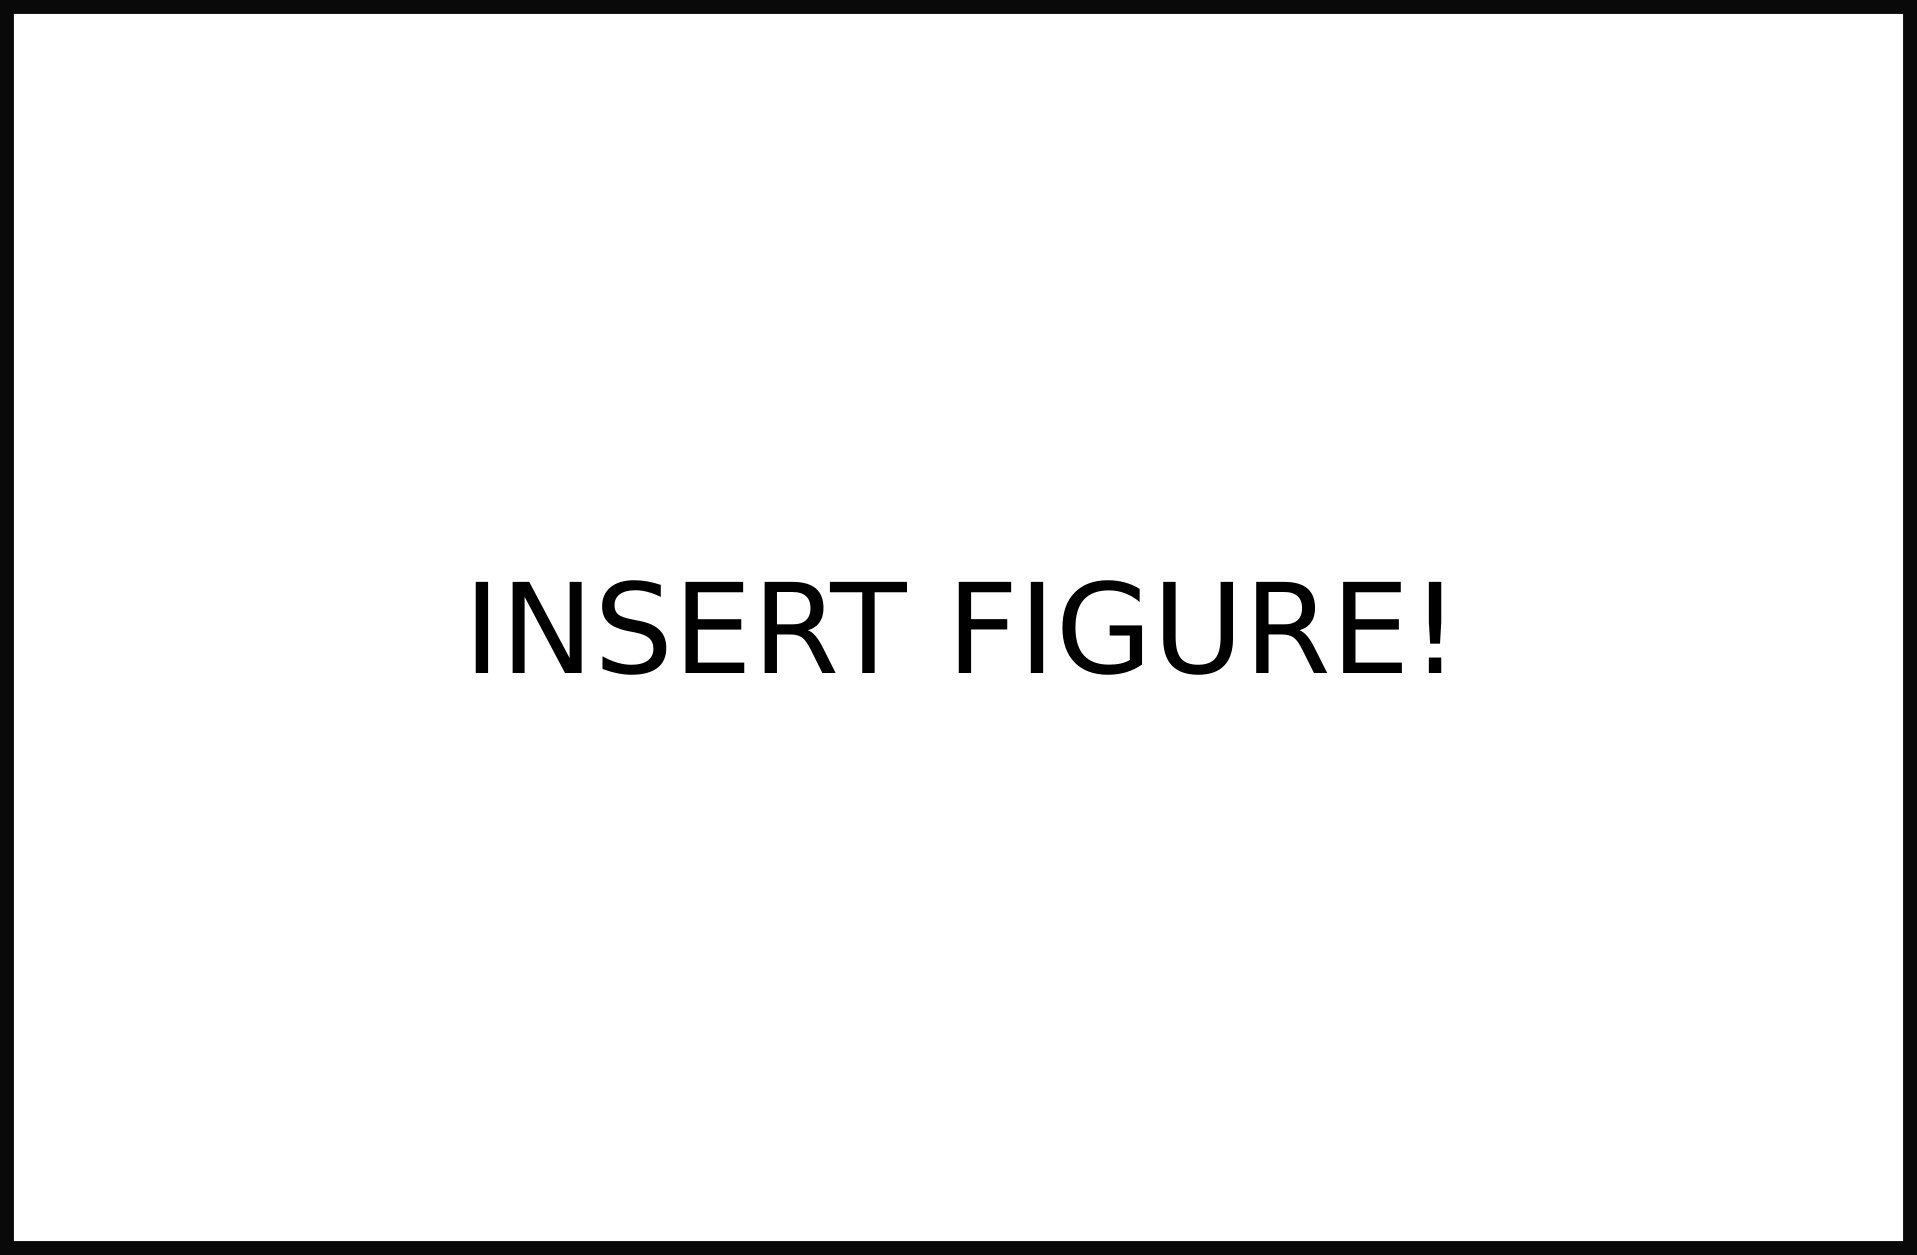
\includegraphics[width=0.8\textwidth]{img/insert_figure_here.png}
\caption[Branching structure of a BnB procedure]{\label{fig:bnb} \textit{Branching structure of a BnB procedure}. What do I write here?}
\end{figure}
% Explaining branch and price
Branch-and-price (BnP) is an extension of the basic BnB. It uses the column generation method to solve the relaxed problems of a BnB tree. The idea of column generation is to only consider a partial set of all optimization variables of the problem. All other variables, which are not explicitly being considered, are set to zero implicitly. This reduces the size of the optimization problem that has to be solved. The challenge with this method is to find the subset of considered variables, whose optimal solution also guarantees an optimal solution of the original problem.\\
Because of it's property to reduce the problem size, BnP is particularly useful for solving bigger optimization problems. However, the nature of the column generation approach requires a certain amount of manual effort to adapt the BnP algorithm to a new problem. While generic BnB solvers are available, this is more difficult to achieve for BnP. Nonetheless, branch-and-price has been increasingly applied to the vehicle routing problem over the recent years.\\ \\
% Examples for the branch and price approach. MAYBE I NEED MORE?
Korsah et al. \cite{korsah_optimal_2010} implements a branch-and-price algorithm for vehicle routing and scheduling problem with precedence and synchronization constraints. The problem setting is motivated by disaster response planning. Different types of rescue vehicles have to be routed optimally to endangered locations. Optimal solutions were obtained for instances up to 20 tasks.

\subsubsection{Evaluation}

Exact solution approaches have the major advantage of being able to produce the globally optimal solution. Even in cases where the optimal solution is not found, they are often able to give lower/upper bound as a result. These bounds at least provide some sort global scale to compare possible solutions with.\\
However, the practicality of exact approaches is severly limited by the subject problem size and complexity. For problem instances with a big amount of elements or constraints, exact methods are often unable to find the optimal solution. Furthermore, they would need a considerable computational effort to produce decent solutions at all.\\
In comparison to other methods, such as metaheuristics, exact methods primarily lack in efficiency. Since this thesis aims to emphasize efficiency (sec. \ref{sec:aim}), exact methods will not be considered in further detail.\\
For further reading on the topic, Blocho \cite{blocho_chapter_2020} presents an introduction in regards to VRP specifically. In his thesis, Meyer \cite{meyer_entwicklung_2019} discusses exact optimization methods in great detail. Additionally, a BnP algorithm is implemented for a heterogeneous multi robot coordination problem.


\subsection{Interactive optimization}\label{sec:interactive}

% I guess I will just make this a general section, which first explains some taxonomies of 
% different classes/types and then jumps into the concrete examples, which I have found
% And I really want to make MAP elites my centerpiece here, because I just really liked the 
% approach a lot!
Interactive optimization is another field, which has been gaining more attention in the recent years. The premise is to design algorithms, which include the human operator into a optimization process to some degree.\\
% MOTIVATING TRUST AS ONE OF THE DRIVING FORCES FOR INTERACTIVE OPTIMIZATION
Some expect the synergy of human heuristic problem solving capabilities and the raw processing power of machines to create even better optimization algorithms. Another, rather pragmatic, advantage of interactive optimization is that of user \textit{trust}. Considering the example of vehicle routing applications, the well-performing optimization algorithms are bundled into some kind of planning software at the end. This software will eventually be used by a human operative in some logistics company. In such a user environment, pure objective value performance is not the only critical factor for the success of a software. If the software only produces a single solution, a human user may be tempted to distrust this solution, if it goes against human intuition. That may even be the case if this unintuitive solution is in fact better exactly because it is not bound to the realm of human logic. Another factor may be, that  there are very human objectives to a planning schedule, which are outside the realm of what can be measured with a simple objective function. An example would be nuanced and temporary driver and customer preferences, which were only defined through personal conversations and are difficult to put into hard numbers. These factors, which contribute to the operators trust into a software/algorithm are addressed by giving the human user an opportunity to contribute to the creation of a solution.\cite{urquhart_increasing_2019} \\ \\
% THE TAXONOMY OF WHICH APPROACHES EXIST
Meignan et al. \cite{meignan_review_2015} compile a review of interactive optimization procedures within the domain of operations research. This review is then used to create a taxonomy of interactive methods, which identifies a total of 5 prominent approaches found within the contemporary literature:
\begin{itemize}
\item \textbf{Trial and error} This is the simplest approach which includes interaction of a human and a system in the context of optimization. The human executes some optimization algorithm, evaluates the result and proceeds to adjust the (hyper-)parameters of the algorithm. This cycle is repeated until a satisfactory solution is found.\\
Despite it's crude nature, this approach has been adapted as a solution to serious problems, as it is illustrated by an example of Meignan et al.: "A more recent approach, based on an interactive trial and-error approach, is presented in Cesta et al. [2003]. This approach deals with the determination of schedules for data transmission from a space probe [...]. The optimization problem consists of determining sequences of data packet transmissions within a set of time frames. It is a variant of the bin packing problem. The problem is modeled as a constraint satisfaction problem and solved using heuristics and metaheuristic search methods. The user can interact with the optimization system, using trial and error, for both adjusting the search strategy and modifying constraints."\cite[p.17:14]{meignan_review_2015}
% provide an example here?
\item \textbf{Interactive reoptimization} The idea of this approach is similar to the trial-and-error method. But instead of completely running the whole optimization again, an initial solution is created and subsequently only changed marginally. The user can make changes to the underlying problem description and the optimization parameters. The algorithm will then also modify the found solution accordingly. Often, an additional objective can be added to the procedure: Aside from optimizing the objective value, the algorithm also has to minimize the 'distance' towards the previous solution. This distance refers to some measure of similarity. This additional objective is added to maintain parts of the solution, which the user does not directly wish to change.
\item \textbf{Interactive multi-objective optimization} Multi-objective optimization in general addresses the issue, that for many problems there are multiple partially conflicting objectives by which to evaluate a solution. A simple aggregation of these objectives might produce suboptimal solutions in regards to some objectives. Thus, the objectives are usually kept separate and have to be treated with specific multi-objective optimization algorithms. In this context, the so called 'Pareto-front' defines a set of solutions, where no improvement is possible in one objective is possible without worsening the value of some other objective. So each point in this set defines a specific trade-off between the individual objectives.\\
This provides a special opportunity for user interaction. The user is able to define the preference towards which particular trade-off is preferred. This process can work much like interactive reoptimization, where an initial solution is created and then the user gradually changes preferences between the different objectives within a loop until a satisfactory result is achieved.
\item \textbf{Interactive evolutionary algorithms} This class of interactive methods focuses on problems, where the objective function is hard to quantify mathematically. It thus addresses problems, which benefit or solely rely on a user's subjective evaluation. The basic idea to incorporate the human into the algorithmic process is to use the user as a substitute for the objective function. For the case of evolutionary algorithms this means, that the standard evolutionary loop of select, crossover and mutate is still executed. But for the evaluation during the selection phase user input is prompted to assign a fitness to the individual solutions. The algorithm then gradually learns which aspects of a solution maximize the user's subjective evaluation.\\
Kim and Cho \cite{kim_application_2000} apply this method for example to the problem of fashion design.
\item \textbf{Human-guided search} The previous methods focused on the user's contribution to changing aspects of the problem or introducing additional constraints. For this method, the idea is for the user to enhance the efficiency of an algorithm. The human is actively involved into the exploration of the search space. This is mostly done by an alternation between a search and a feedback phase. During the feedback phase, the user assigns penalty-like values to some aspects of a solution, which are aimed at restricting and thus focusing the search. The algorithm then included mechanisms in the search phase which prevent from descending into high-penalty areas of the search space.
\end{itemize}
% SMALL OVERVIEW OF NEXT TOPICS TO NOT CONFUSE THE READER
The following paragraphs will go into slightly more detail regarding one recent example of interactive vehicle routing optimization. This detailed example is supposed to provide a small insight into the general idea of interactive techniques.\\
The section will then continue by providing referential examples of interactive procedures within the broader context of vehicle routing applications. The list of these examples is not intended to be exhaustive and most likely does not include the most relevant works. It was examples, which have popped up during a brief scan of the literature.\\ \\
% BRINGING UP MAP ELITES AS A SPECIFIC EXAMPLE
Urquhart et al. \cite{urquhart_optimisation_2018}, \cite{urquhart_using_2020} proposed a technique called 'MAP-elites' to be applied to the workforce scheduling and routing problem. MAP-elites is an algorithm, which was proposed by Mouret and Clune \cite{mouret_illuminating_2015}. It is not classified as a traditional search/optimization algorithm, but has been called an illumination algorithm. The goal is not to find a single best solution, but rather to provide an overview of how high-performing individual solutions are distributed over the search space. This algorithm was originally introduced for optimization within engineering design problems, such as electronic circuit design, automated scientific discovery or artificial intelligence.\\
Urquhart et al. transfered the idea to the realm of vehicle routing. Their basic setup includes the definition of one main objective function as well as multiple, potentially conflicting, secondary objectives for the optimization of the WSRP. In their work they consider for example the total travel cost and the total employee cost among others. For both of these objectives, separate evaluation functions would be defined. The value of these objectives is then considered to be along the axis if a coordinate system. This continuous coordinate system is then furthermore divided into discrete bins. The result is a discrete coordinate system consisting of a number of 'tiles'. The core optimization procedure is a genetic algorithm, which is maintaining a population of solutions to iteratively execute the evolutionary cycle. The main change is within the evaluation phase: Each solutions is evaluated for the main objective as well as for every secondary objective as well. The values of these secondary objectives are then used to assign it to one specific bin. If there is no solution in this bin yet, it will be deposited directly. If there already exists a solution, it will be replaced only if the main objective value of the new solution is better. Like this the population will be distributed among the bins. Over time, only the best solutions in regards to their main objective will remain in this 'archive of elites'. An illustrative example can be seen in figure \ref{fig:mapelites}. This example shows how the results of the algorithm may be presented to a user. The interactivity stems from the fact that it is finally the users choice, which solution will be finally implemented. The archive presents all necessary information. Specifically it illustrates well, how a choice of extreme secondary objective values corresponds with a particular trade-off towards the main objective.\\ \\
% FIGURE WHICH SORT OF ILLUSTRATES THE STRUCTURE OF THESE ARCHIVES
\begin{figure}
\centering
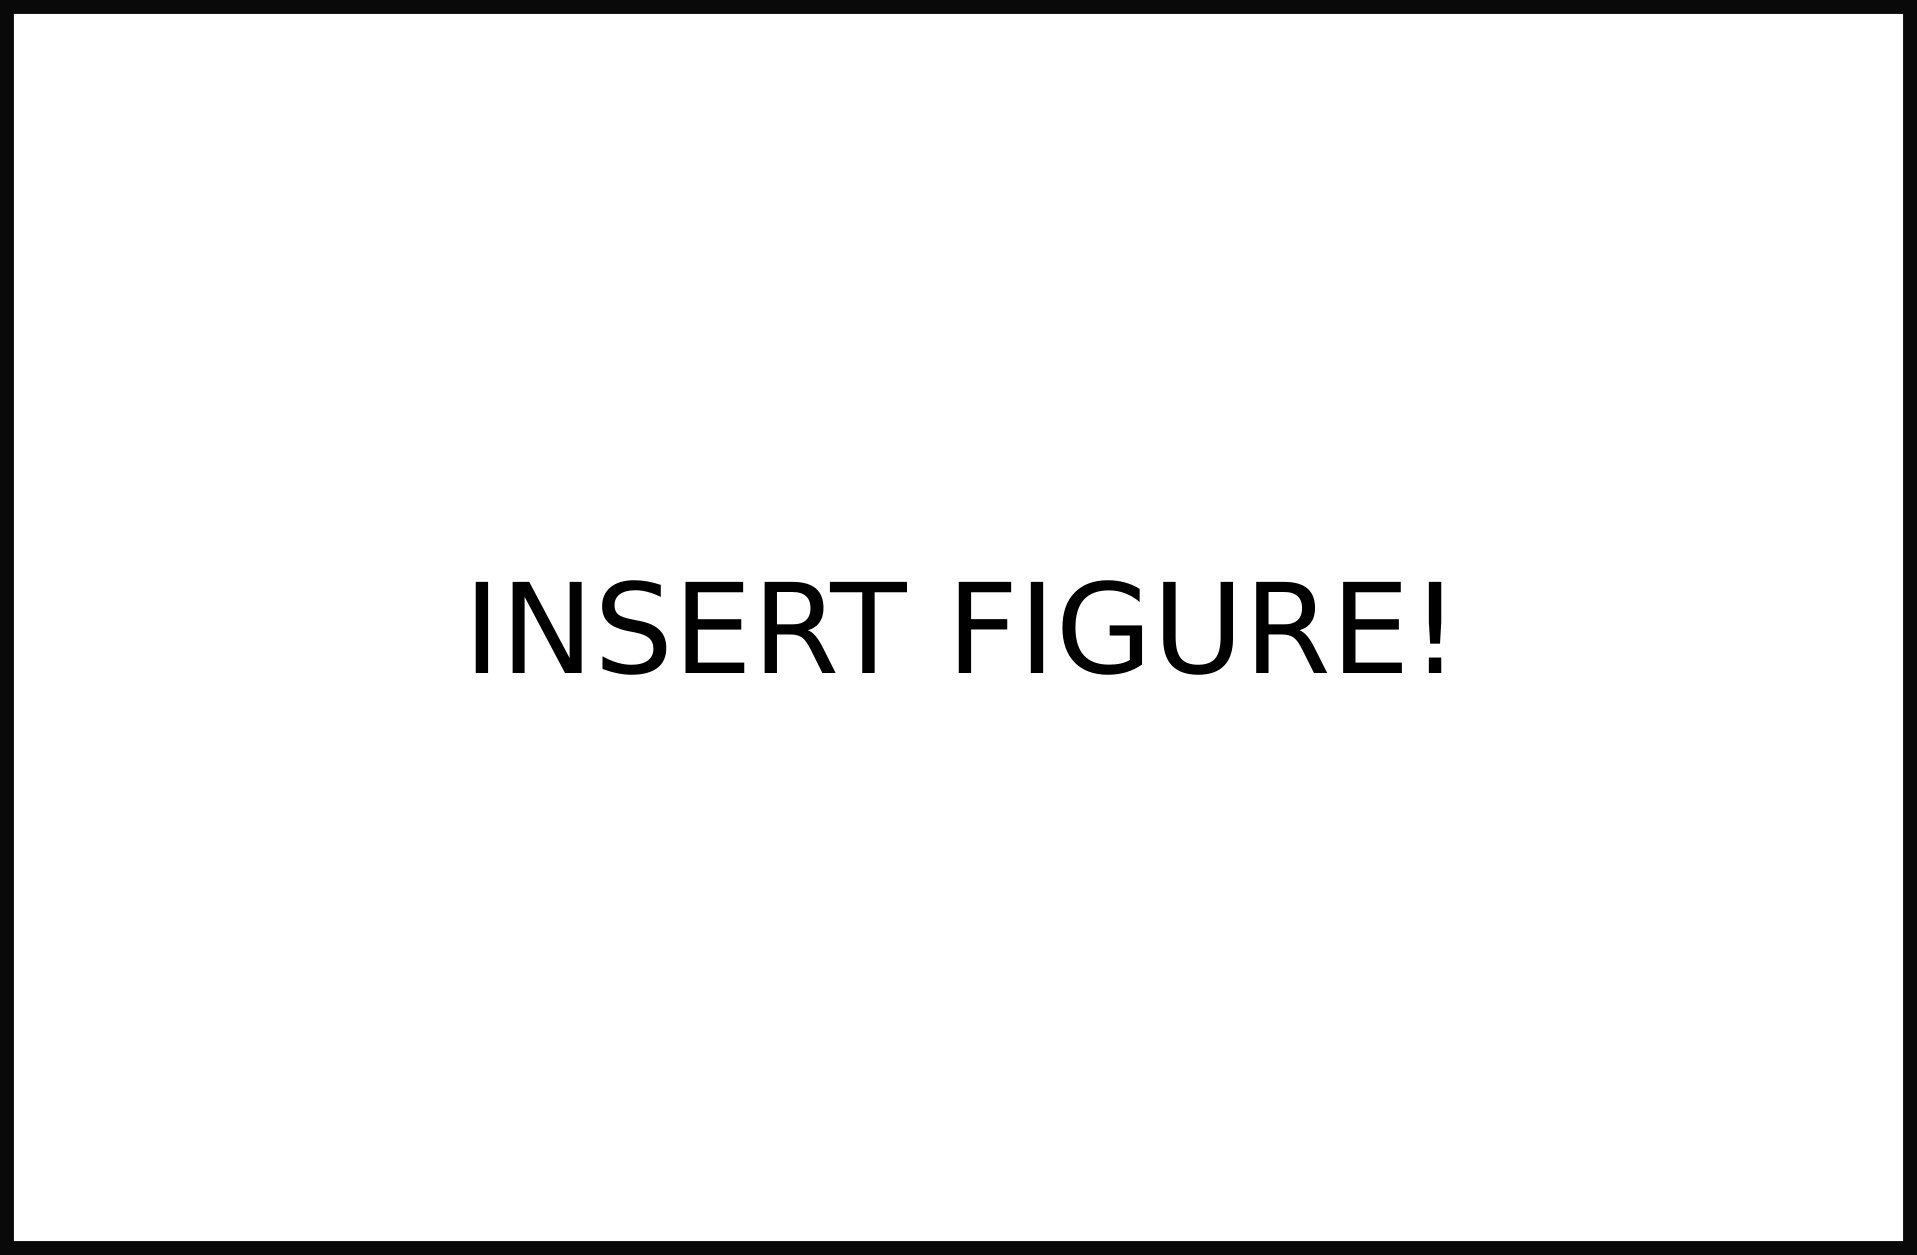
\includegraphics[width=0.8\textwidth]{img/insert_figure_here.png}
\caption[Example of a MAP-elites archive]{\label{fig:mapelites} \textit{Example of a MAP-elites archive}. This figure shows an illustrative example of how the solution of a MAP-elites algorithm may look like. This example assumes that there are only two secondary objectives, hence this is a two-dimensional coordinate system. Darker shades of green imply a better main objective value. A white tile indicates, that no solution with fitting values has ever been found.}
\end{figure}
% NOW FOR OTHER EXAMPLES OF INTERACTIVE TECHNIQUES
Yan et al. \cite{yan_human_2016} proposed a cooperative brain storm optimization algorithm for the two-echelon vehicle routing problem. The two-echelon VRP is a special case of the HVRP and the brain storm optimization (BSO) can be seen as a kind of population based metaheuristic. They are able to confirm a basic feasibility of the technique, but admit that the interactive approach still needs refinement.\\
Bossek et al. \cite{bossek_towards_2020} design a dynamic evolutionary multi-objective algorithm for the bi-objective vehicle routing problem. A decision-maker makes a decision about the priority of the objectives during each generation of the evolution. In this preliminary approach human interaction was replaced with different artificial decision strategies. Nonetheless, the effectiveness of the approach was demonstrated, although there is much opportunity for further improvements.\\
Kim et al. \cite{kim_collaborative_2017} presents a work which aims to achieve collaborative planning by encoding user's high-level strategies. Several users were asked to articulate their high-level strategies for solving a planning problem. These were then manually translated into a planning language and included in a computational search algorithm. The considered planning problems were various multi-vehicle routing and task allocation problems. The achieved results were comparable to previous benchmarks on the dataset and most of all showed high similarity to the results of the human planners themselves, thus increasing solution interpretability.

\subsubsection{Evaluation}

Interactive optimization methods aim to increase human trust into the results of an optimization process. Furthermore they seek to harness the heuristic human problem solving capabilities to further refine existing computational approaches. Both of these aspects make for interesting directions of further research. For this thesis however, the aspect of user trust is out of scope in regards to the previously defined aim. Additionally, interactive approaches do not seem to yet have significantly improved performance in comparison to the best traditional approaches.\\
Due to these reasons, the interactive approaches will be excluded from further investigation within this thesis.

\subsection{Others}\label{sec:others}

% Make this brief! Just quickly talk about Hyperheuristics and Mix forms etc.

hyperheuristics, matheuristics. I need to research this basically completely from scratch

\newpage


\section{Approaches for solving multi-robot coordination problems}\label{sec:mrta-approaches}

% 27.05.2020
% I think this section needs an introduction, where I tell that this section is not very in depth
% it is only supposed to provide a little insight into how things are being done in a different field.

% Quickly explaining why this section looks the way it looks
This section will briefly introduce the approaches and algorithms which are commonly used to solve the multi robot coordination problem. For this purpose it is important to emphasize the results of section \ref{sec:problem-comparison}. The VRP and MRTA problems share a lot of similarities. As such similar problems, a lot of the common solution approaches are naturally also very similar. The basic metaheuristic algorithms applied to MRTA are the same as for the VRP. This is why the results of these previous sections will not be repeated here.\\
Instead, this section will mainly focus only on those aspects which are different from the field of vehicle routing. This main difference in the basic approach to solving the respective problems can be summarized like this: Vehicle routing approaches have been traditionally static. The applications of the VRP involved the separation of a planning phase and an execution phase. The dynamic VRP, which involves the adjustment of the plan to dynamic changes of circumstances, is a rather novel concept in comparison. For MRTA, this is a little bit different. The dynamic nature of an environment is considered much more often. Hereby, the class of 'instantaneous assignment' (see sec. \ref{sec:mrta-taxonomy}) problems is mainly concerned with the challenge of producing plans without prior knowledge of future events.\\ \\
% How this section is organized
This section is thus organized into two main categories: Section \ref{sec:instant-assign} deals with solutions for the instantaneous assignment problem. Section \ref{sec:extended-assign} will be about the time-extended assignment problem. Since this section will be more similar to the VRP, it will only briefly address MRTA examples for those methods and algorithms, which have been discussed previously throughout section \ref{sec:vrp-approaches}.

\subsection{Instantaneous assignment}\label{sec:instant-assign}

% I could mention that this is much more common in the MRTA
% And a trend for solving these is auction based methods...

\subsection{Time-extended assignment}\label{sec:extended-assign}

\subsubsection{Exact solution approaches}

% Korsahs dissertation.

\newpage

% 22.05.2020
% This section is supposed to showcase the usage of the MAP Elites algorithm to solve the optimisation problem
% I could really include all the papers I have found here. I could start of with a general explanation of what 
% MAP elites are, where they come from. Then the explanation of how it has been used for the WSRP. Then I could 
% mention that it is really promising due to the fact that it would increase the trust into an algorithm and 
% I could finish the section with an outlook of how to potentially improve the approach in the future based on 
% the improvements to the classic MAP-Elites algorithm.

%\newpage
%\section{Related Work} \label{sec:related-work}

% 18.05.2020
% So what this section is supposed to be about:
% I want to give a rough overview of how different, specfic VRP research domains relate to the the relevant problem.
% At first I intended to also sort of talk about this sort of thing in the "Existing solutions" section, but then 
% two things happenend:
% 1: I realized that the existing solutions section will get way bigger on its own already.
% 2: I read the castello phd and realized, that there are multiple other fields, which were also related to the problem 
% and then the whole section would just have been to big

% Currently, at the time of writing this, I only really have solid information on the HHC and some info on the TTSP 
% So thats also some things I might have to keep researching.

%\subsection{Home Health Care} \label{sec:hhc}

% \subsection{Technician Scheduling} \label{sec:ttsp}

% \subsection{Manpower Allocation} \label{sec:mtap}

% \subsection{Worforce Routing and Scheduling} \label{sec:wrsp}


\section{Existing solutions} \label{sec:selected}

% 08.05.2020
% So my initial idea for this section was to have one giant table, which lists the most promising papers and all their 
% features in varing degrees of sophistication.
% But after thinking about it more I have come to the realization, that papers themselves are so different in each of 
% the attributes, that by putting it all into a single table with just symbols differentiating their differences I would 
% loose a lot of information for one thing and additionally it would probably be so cluttered, that it would be hard to 
% make any sense of it at all.
%
% My other idea would be to have separate sections and also separate tables comparing the papers regarding all these 
% different attributes first and then having this big ass summary table, much as I have conceptionalized it before maybe 
% even later in the evaluation section. On the basis of this summarizing comparison I would then argue for my choice of 
% which approach probably suits the purpose best.  
%
% So I guess thinking about this idea I would start of with a table, which would list all the papers and some general 
% informations about them. Like what field they are from, what algorithmic approach they have taken, how they have 
% verified their solutions (which test instances where used and such). In the acompaning text I could just roughly describe 
% the general idea, maybe also behind the algorithms which they are using.
%
% Then I would need such sections of "precedence & cooperativity", "Heterogeneity" and "Objective Function". In each of 
% these sections I would first describe that the papers are handeling it very differently then describe my criteria for 
% ranking them and provide a table with that comparison followed by an in depth explanation of what potentially 
% makes them special...

% REDO THIS!
The following section showcases selected, concrete approaches from existing VRP literature, which exert favorable attributes for being applied to the subject multi robot coordination problem.\\
At first, two sub-areas of the well known VRP are presented in sections \ref{sec:hhc} and \ref{sec:ttsp}. These areas will be highlighted due to their collective recent focus on synchronization constraints, as presented in section \ref{sec:sync}.\\
Then individual publications and their approaches will be showcased and compared in respect to their implementation of the favorable attributes. These favorable attributes being the ones identified in section [?] as crucial for a most complete representation of the multi robot coordination problem motivated by planetary exploration and mission planning. These criteria include the possibility of cooperative task execution, precedence constraints and agent heterogeneity.\\
The section will close with an evaluation of the presented literature and their characteristics. Based on this evaluation of the the presented approaches, one will be chosen for further investigation within this thesis.

% I feel like this deserves a spot here, because the multi robot problem is at its core more of a scheduling problem
% than a routing problem. TTSP also is a scheduling problem which is


\subsection{Comparison of selected approaches}

% 08.05.2020
% OK so this paragraph will gently introcude all of the approaches by name. The question here is in which order or better
% by what criteria would I cluster them. I could do them chronologically but that would have the problem of maybe having 
% a few sentences out of context. I could cluster them also by what approach they where following or by how the problem 
% formulation is structured...
%
% I guess I am going to opt for the first level of clustering being the problem, which is being solved. Which would be 
% smth. like the HHC or the TTCP etc. And then within the HHC most notably I would go a little bit with a logical order of 
% what came first and what made which incremental improvements.

% Make it simpler
This selection of publications has been made based on their varying degrees of sophistication regarding the criteria of homogeneity, cooperativity, precedence, objective function, time windows and algorithm performance. The presented subset is not assumed to be complete. Some problem characteristics and/or approaches are vastly widespread in the broader field of VRP literature. For such cases, presenting all or even multiple possible solutions would exceed the scope of this comparison. Furthermore, in such a case the chosen publications are exemplary for the characteristics of their respective fields.\\
The selection does however contain all the singular outstanding publications, which have revealed themselves to be the most promising subjects regarding an adaption to the multi robot problem.\\

%
% So I thought that maybe before I start the whole detailed description here I could make a little remark about the fact
% that most of of the relevant publications are from the home health care problem. I think I dont need to be too in depth
% because I feel like I am going to mention this at some place else as well....
%
Bredström and Rönnquvist \cite{bredstromCombinedVehicleRouting2008a} present a MIP model formulation for the Vehicle Routing and Scheduling Problem with time windows and additional temporal constraints. By doing so they are one of the first to introduce the idea of pairwise synchronization and precedence constraints to the vehicle routing problem. They argue, that temporal dependencies between tasks are more expressive in describing real life problems. As an example they mention the issues of homecare staff scheduling and forest operations, which both exert strong requirements of task interdependency. The problem is solved using a MIP-based decomposition heuristic.\\
%
Rasmussen et al. \cite{rasmussenHomeCareCrew2012} consider the Home Care Crew Scheduling Problem with soft preferences and temporal dependencies. In this problem a set of home carers, such as nurses, has to be assigned to a given set of services at patients homes to minimize the total operational cost as well as negative patient preference for individual home carers. Pairwise synchronization and precedence constraints are considered between services. A Branch-and-Price algorithm is developed to solve smaller instances to optimality. For large instances preference-based visit clustering is employed to reduce problem complexity and thus computational time.\\
%
In Mankowska et al. \cite{mankowskaHomeHealthCare2014} the problem of Home Health Care Routing and Scheduling is also investigated. Pairwise synchronization and precedence are also considered, although allowing only a maximum of two interdependent services per node/patient. Additionally they consider home carers with heterogeneous sets of qualifications, but no patient preferences. They propose an Adaptive Variable Neighborhood Search algorithm, which adjusts the search tree exploration strategy specific to the concrete problem instance.\\
%
Ait Haddadene et al. \cite{aithaddadeneGRASPILSVehicle2016} also work on the problem of Home Health Care Routing and Scheduling. Aside from preferences and temporal dependencies, heterogeneous qualifications and multiple service patients are used for the model. They evaluate GRASP and ILS metaheuristics as well as a hybrid approach of the former for solving the proposed MIP model and confirm the hybrid algorithm to be superior to the single solutions.\\
In a different work \cite{haddadeneNSGAIIEnhancedLocal2016} the same researchers investigated the problem using a true multi-objective approach to simultaneously optimize the total travel time of home carers as well as patient preferences. They employed different variations of the Non-dominated Sorting Genetic Algorithm enhanced with local search to solve the bi-objective problem. The conclusion yields, that while the approach efficiently solves the problem, no substantial improvement could be made.\\ % This is kind of a bold move to say that here, but thats sort of what I am taking away from their paper. Also is it clear, that this is my assessment of the thing and not literally what they are saying in the conclusion 
%
Lasfargeas et al. \cite{lasfargeasSolvingHomeHealth2019} try to solve the home Home Health Care problem with temporal synchronization and precedence between tasks as well. Aside from worker qualifications they also introduce hard patient as well as worker preferences. They argue, that both patients as well as workers might have incentives to refuse some workers and patients respectively. For patients social embarrassment regarding nurses of the opposite sex would be an example. Likewise nurses suffering from serious allergies could avoid visiting the homes of pet owners. The objective is to minimize a weighted sum of all the job starting times, and time window violations, while also considering worker break time regulations. A possible solution to the problem is provided by a novel construction heuristic and a Variable Neighborhood Search metaheuristic.\\
%
Manavizadeh et al. \cite{manavizadehUsingMetaheuristicAlgorithm2020} propose a MILP model for the Home Health Care Problem which considers staff qualification and multiple interdependent services per patient. In this case the problem is also designed with an unlimited number of possible home carers. For each additional home carer employed in the final schedule a fixed cost is added to the overall objective function. So aside from minimizing the total travel cost and time window violation the objective also considers to minimize the total amount of home carers required. A big part of of the work is dedicated to a sensitivity analysis of the proposed model in regards to several instance parameters. A commercial solver is used for small and medium sized problem instances and a Simulated Annealing algorithm is devised to solve larger instances.\\
%
The model proposed by Entezari and Mahootchi \cite{entezariDevelopingMathematicalModel2020} also supports temporal precedence and synchronization, as well as worker qualifications for the Home Health Care Problem. The objective function included terms for total travel distance, time window violations, home carer working hour violations and patient preferences. Additional constraints are introduced to support break time regulations for workers and optional retrieval of blood samples from the patients homes. A genetic algorithm is developed to solve the problem.\\ \\ 
% Now here begin the other papers, which are not about the home health care problem
Korsah et al. \cite{korsahOptimalVehicleRouting2010} introduce a MIP model for the Vehicle Routing Problem, which handles task synchronization and precedence, heterogeneous vehicle capabilities and location choice. The application of the proposed model is motivated by disaster preparedness planning. In the case of a natural disaster support vehicles can be routed efficiently to provide medical attention and evacuate the population. The novel addition of location choice introduces the idea that a given task does not have to be performed at a single location, but at a set of possible locations. An optimal solution algorithm based on the branch-and-price framework is developed to fit the specific model.\\
%
Tao et al. \cite{taoMetaheuristicAlgorithmTransporter2019} is motivated by transporter scheduling for assembly blocks in a shipyard. The problem is modeled as a multiple Traveling Salesman Problem with synchronization and precedence constraints. Transport vehicles are however modeled with homogeneous capabilities. The objective is to minimize a total of all transport, delay and waiting times. A hybrid Genetic algorithm and Tabu Search subprocedure is developed to solve the problem.\\
%
% Maybe mention that this was the winning algorithm for the ROADEF challange
Firat and Hurkens \cite{firatImprovedMIPbasedApproach2012} present a model for the Multi-Skill Technician Task Scheduling Problem, in which a set of technicians with heterogeneous skill levels in different domains is partitioned into teams on a daily basis to complete a set of tasks. These tasks may require varying degrees of skills and they may define precedence relationships towards other tasks, as well as priorities. The most notable difference of this approach to all previously mentioned is that neither a spatial routing aspect nor time windows are considered for the problem. A combinatorial algorithm is developed for the model. This approach brought forth the best overall solutions for the ROADEF challange \cite{dutotTechniciansInterventionsScheduling2006}\\
%
Pereira et al \cite{pereiraMultiperiodWorkforceScheduling2020} also work on an extension of the TTSP, denoted Multiperiod Worforce Scheduling and Routing Problem. They introduce a routing aspect to the original scheduling problem by defining travel distances as arc weights in a graph of task nodes. Tasks may consist of subtasks, which can define precedence relationships. Additionally these subtasks can also define skill requirements for the processing team, although team composition is assumed to be fixed throughout the multiperiod planning horizon. The objective is to minimize the final day of the schedule. A novel construction heuristic along with multiple variations of the Ant Colony Optimization metaheuristic are evaluated for their effectiveness for solving the problem.\\ \\
%
% 06.06.2020
% I have moved this table from the actual main Literature.tex file to its own file

% While formatting this table I have noticed, that "problem" column is pretty obsolote. It does not really provide any 
% kind of useful information, since most of these papers do not define a strict problem formulation.
% I have been thinking to change the column to "problem field" and provide info about how the formulation is 
% motivated such as "home health care problem" or "worforce scheduling and routing" etc. This would provide more 
% information than how it is now.

% Look at this resource if at any point there are problems with the center allignment of the items...
% https://tex.stackexchange.com/questions/341205/what-is-the-difference-between-tabular-tabular-and-tabularx-environments
\begin{table}[t]
	\tableConfig
	\begin{tabular*}{\textwidth}{@{\extracolsep{\fill}}lllllrl}
		% BEGIN TableHead
		\toprule
		% FirstHeadRow
		\multicolumn{2}{l}{Publication} 									&
		\multicolumn{3}{l}{Characteristics} 									&
		\multicolumn{2}{l}{Computational tests} 								\\
		\cmidrule(rl){1-2} \cmidrule(rl){3-5} \cmidrule(rl){6-7}
		% SecondHeadRow		
		\multicolumn{1}{l}{Reference} 										&
		\multicolumn{1}{l}{Year} 										&
		\multicolumn{1}{l}{Field} 										&
		\multicolumn{1}{l}{Approach} 										&
		\multicolumn{1}{l}{Optimal?} 										&
		\multicolumn{1}{l}{$|N|^{(a)}$} 									&
		\multicolumn{1}{l}{Instance origin} 									\\
		\midrule %
		% END TableHead
		%
		% ------------------------------------------------------------------------------
		%
		% BEGIN TableContent
		\cite{bredstromCombinedVehicleRouting2008a} & 
			2008 & 
			Home Health Care & 
			MIP heur. &  
				& 
			80 & 
			random \\
		%
		\cite{rasmussenHomeCareCrew2012} & 
			2012 & 
			Home Health Care & 
			BnB & 
			\yes$^{(b)}$ & 
			150 & 
			real world data \\
		%
		\cite{mankowskaHomeHealthCare2014} & 
			2014 & 
			Home Health Care & 
			AVNS & 
				& 
			300 & 
			random \\
		%
		\cite{haddadeneNSGAIIEnhancedLocal2016} & 
			2016 & 
			Home Health Care & 
			NSGAII & 
			 & 
			73 & 
			\cite{bredstromCombinedVehicleRouting2008a} \\
		%
		\cite{aithaddadeneGRASPILSVehicle2016} & 
			2016 & 
			Home Health Care & 
			GRASPxILS & 
			 & 
			73 & 
			\cite{bredstromCombinedVehicleRouting2008a} \\
		%
		\cite{lasfargeasSolvingHomeHealth2019} & 
			2019 & 
			Home Health Care & 
			VNS &  
			 & 
			300 & 
			\cite{mankowskaHomeHealthCare2014} \\
		%
		\cite{manavizadehUsingMetaheuristicAlgorithm2020} & 
			2020 & 
			Home Health Care & 
			SA &  
			 & 
			250 & 
			random \\
		%
		\cite{entezariDevelopingMathematicalModel2020} & 
			2020 & 
			Home Health Care & 
			GA &  
			 & 
			50 & 
			random \\
		%
		\cite{korsahOptimalVehicleRouting2010} & 
			2010 & 
			Disaster response & 
			BnP & 
			\yes & 
			20 & 
			random \\
		%
		\cite{taoMetaheuristicAlgorithmTransporter2019} & 
			2019 & 
			Construction & 
			GAxTS & 
			 & 
			50 & 
			random \\
		%
		\cite{firatImprovedMIPbasedApproach2012} & 
			2012 & 
			Technician Scheduling & 
			Constr. heur. & 
			 & 
			800 & 
			\cite{dutotTechniciansInterventionsScheduling2006} \\
		%
		\cite{pereiraMultiperiodWorkforceScheduling2020} & 
			2020 & 
			Technician Scheduling & 
			ACO & 
			 & 
			100 & 
			random \\
		%
		\bottomrule
	\end{tabular*} 
	\caption[Overview of selected publications]{%
		\label{tab:initial-compare}% 
		\textit{Overview of selected publications}. The table shows the following columns enumerated from left to right: (1) A reference to the specific paper, (2) the year it was published, (3) an abbreviation for the name of the problem which was addressed in the paper, (4) the name of the algorithm/approach used to solve the problem, (5) whether or not optimal solutions could be produced with this approach, (6) the number of nodes for the largest studied problem instance and (7) the origin of the problem instances used.%
\footnoterule
%
\hspace*{0.2cm}{$^{(a)}$It is important to note, that the problem complexity is dependent on a multitude of other things beside the number of nodes. Examples would be the number of vehicles and the density of synchronized visits. The parameter for the amount of nodes presented here is only meant to provide a first impression of the problem complexity.}\\ %
%
%\hspace*{0.2cm}{$^{(b)}$The "Home Health Care Problem" and other synonymous terms are not consistently representative of a specific problem formulation throughout the literature. Thus all publications dealing with the general problem of home health care have been summarized here.}\\ %
%
\hspace*{0.2cm}{$^{(b)}$An optimal algorithm is developed, but to reduce computational times it is extended wit a heuristic clustering method for larger instances, thus loosing optimality.}}
\end{table}

%
% So the next section is supposed to reference the table 
% How in depth does this have to be. Do I really have to spell out which columns of the 
% table i am specifically refering to or can I just assume the reader can conclue this themselves
Table \ref{tab:initial-compare} provides an overview of the selected publications. For each presented work it contains the information about which problem is to be solved, the chosen approach to solve the problem and whether or not this approach is able to produce optimal results. Additionally some information about the computational testing is provided with the number of nodes within the largest processed problem instance and the origin of the used set of problem instances.\\
From this overview some initial observations can already be made:\\
\textit{Instance sizes.} Problem instances for computational testing tend to be comparably small with a cap of 300 nodes. Only Firat and Hurkens \cite{firatImprovedMIPbasedApproach2012} presents itself as an outlier, managing up to 800 tasks within the biggest instance. Regarding this specific paper, it has to be emphasized that the underlying problem studied in their work is purely scheduling based and does not contain a routing component.\\
\textit{Heuristic approaches.} Most of the relevant literature seems to prefer heuristic and metaheuristic approaches over those with the capability to provide globally optimal solutions. The two approaches presented here which actually do implement optimal procedures, namely \cite{korsahOptimalVehicleRouting2010} and \cite{rasmussenHomeCareCrew2012}, are only able to handle even smaller problem instances. Korsah et al. \cite{korsahOptimalVehicleRouting2010} only handles instances with up to 20 nodes. Rasmussen et al. \cite{rasmussenHomeCareCrew2012} indeed handle larger instances with a size up to 150 nodes, although only by using a clustering-enhanced branching scheme and thus loosing global optimality.\\
\textit{Problem instances.} Regarding the origin of the problem instances used for computational testing there are mainly two basic options: Using real world data, which was provided for example by an actual home health care provider, or randomly generating data sets. Most often, the random generation of data sets is also designed in such a way that the final results best reflect actual circumstances for the motivated real life domain. This could for example include a certain spatial clustering of nodes or a specific ratio of single versus synchronized visits. Within the reviewed literature this generation of data seemed to be the more popular choice.\\
Another prominent option for handling computational tests is to use instances from other publications. This is often done to be able to compare the performance of a new algorithm to other earlier solutions within the literature in respects to objective function value and/or computational time. For this aspect it can be noted that both the original instances of Bredström \& Rönqvist \cite{bredstromCombinedVehicleRouting2008a} and Mankowska et al. \cite{mankowskaHomeHealthCare2014} have occasionally been reused throughout more recent publications.

\subsubsection{Precedence and Cooperativity}

% I think as a first section I want to do a little recap of what these words mean
% and also why they are important
The following section will compare the selected publications regarding their characteristics of precedence and cooperativity.\\
The criteria of precedence describes the ability of an approach to be able to handle additional constraints, which link two or more tasks into a precedence relationship. One such constraint expresses the need that certain tasks need to be started or completed before work on another task can start.\\\cite{korsah_comprehensive_2013}
The criteria of cooperativity, in the following used synonymously with the term \textit{synchronization}, refers to the potential need of one or more robots cooperating to solve a task together. Including this option opens up a myriad of possibilities for problem solving. Especially in combination with heterogeneous robot fleets, this enables the cooperation of multiple specialized abilities to perform more complex tasks.\\
%
% 26.05.2020
% So here is what I have found out about these damned table environments in latex:
% - Using the "supertabular" environment within a "table" does not work because 
% supertabular is designed in a way, that supports line breaks, but the table does not support this at all and attempts to put the 
% potentially two separate sections onto the same page. That causes a pretty big problem.
% Although I did not test out what happens if I make an empty but otherwise staticly sized \tablehead to compensate the jankyness of 
% the second part...
% But its a good idea to just use supertabular within a "center" environment...
% - The tabular environments using the asterisk at the end "supertabular*" and "tabular*" are designed to not have a fixed width.
% They expect an additional parameter which will set this width \begin{supertabular}{\textwidth}{llc} for example
% - This IRS latex template cannot use the package "xtabs", because the symbols page has been designed with supertabular and these 
% two packages conflict with each other. And changing the symbols page would be way too much effort. So I will be stuck with 
% supertabular..

% Look at this resource if at any point there are problems with the center allignment of the items...
% https://tex.stackexchange.com/questions/341205/what-is-the-difference-between-tabular-tabular-and-tabularx-environments
\begin{table}[t]
	\tableConfig
	\begin{tabular*}{\textwidth}{@{\extracolsep{\fill}}lccccccc}
		% BEGIN TableHead
		\toprule
		% FirstHeadRow
		\multicolumn{1}{l}{} 								&
		\multicolumn{4}{l}{Cooperativity} 					&
		\multicolumn{3}{l}{Precedence} 						\\
		\cmidrule(rl){2-5} \cmidrule(rl){6-8}
		% SecondHeadRow		
		\multicolumn{1}{l}{reference} 						&
		\multicolumn{1}{l}{at all?} 						&
		\multicolumn{1}{l}{between nodes?} 					&
		\multicolumn{1}{l}{>2?} 							&
		\multicolumn{1}{l}{Team building?} 					&
		\multicolumn{1}{l}{at all?} 						&
		\multicolumn{1}{l}{between nodes?} 					&
		\multicolumn{1}{l}{$\delta_{min}, \delta_{max}$} 	\\
		\midrule %
		% END TableHead
		%
		% ------------------------------------------------------------------------------
		%
		% BEGIN TableContent
		\cite{bredstromCombinedVehicleRouting2008a} & 
			\yes & 
			\yes & 
			\yes &  
			 & 
			\yes & 
			\yes & 
			\yes \\
		%
		\cite{rasmussenHomeCareCrew2012} & 
			\yes & 
			\yes & 
			\yes & 
			 & 
			\yes & 
			\yes & 
			\yes \\
		%
		\cite{mankowskaHomeHealthCare2014} & 
			\yes & 
			 & 
	  		 & 
			 & 
			\yes & 
			 & 
			\yes \\
		%
		\cite{haddadeneNSGAIIEnhancedLocal2016} & 
			\yes & 
			 & 
			\yes & 
			 & 
			\yes & 
			 & 
			\yes \\
		%
		\cite{aithaddadeneGRASPILSVehicle2016} & 
			\yes &
			 & 
			\yes &
			 & 
			\yes & 
			 & 
			\yes \\
		%
		\cite{lasfargeasSolvingHomeHealth2019} & 
			\yes & 
			\yes & 
			\yes &  
			 & 
			\yes & 
			\yes & 
			\yes \\
		%
		\cite{manavizadehUsingMetaheuristicAlgorithm2020} & 
			\yes & 
			\yes & 
			\yes &  
			 & 
			\yes & 
			\yes & 
			\yes \\
		%
		\cite{entezariDevelopingMathematicalModel2020} & 
			\yes & 
			\yes & 
			\yes &  
			 & 
			\yes & 
			\yes & 
			\yes \\
		%
		\cite{korsahOptimalVehicleRouting2010} & 
			 & 
			 & 
			 & 
			 & 
			\yes & 
			\yes & 
			 \\
		%
		\cite{taoMetaheuristicAlgorithmTransporter2019} & 
			\yes & 
			\yes & 
			\yes & 
			 & 
			\yes & 
			\yes & 
			 \\
		%
		\cite{firatImprovedMIPbasedApproach2012} & 
			\yes & 
			 & 
			\yes & 
			\yes & 
			\yes & 
			\yes & 
 			 \\
		%
		\cite{pereiraMultiperiodWorkforceScheduling2020} & 
			\yes & 
			 & 
			 & 
			 & 
			\yes & 
			\yes & 
			 \\
		%
		\bottomrule
	\end{tabular*} 
	\caption[Precedence and Cooperativity characteristics of selected publications]{%
		\label{tab:coop-prec-compare}\textit{Precedence and Cooperativity characteristics of selected publications}. %
		% 
		Columns of the table contain the following content (enumeratied from left to right): (1) A reference to the publication in question (2) If there is any concept of cooperativity (3) If cooperative task execution is defined between pairs of nodes (4) If cooperative behaviour can include more than two robots (5) If cooperativity is implemented by team building (6) If there is any concept of precedence (7) If precedence relationships are defined between nodes (8) If the precedence formulation includes a minimum and maximum starting time distance %
		}%
\end{table}

%
% So this section here will mention the table and explain the choices of the chosen criteria
% It will be something like, yeah not everyone implements Cooperativity the same there could be this and that
% The next section after that then will probably deal with the indivdiual papers batch wise. 
% Because some of the papers build on one another and use the same formulation etc so I can easily just mention them in the same context.

% I guess in the end I also need a "recap" or something where I can 


\subsubsection{Heterogeneity}

tbd
%
% 06.06.2020
% Created this table

% The table head looks a little bit weird with the different column levels. I'll have to ask if this is ok.
% An idea would be to append another level 2 column at the end "secondary" Which is either travel costs or other and 
% if the other is not checked then this would imply that there is no sense of heterogeneity.

% Look at this resource if at any point there are problems with the center allignment of the items...
% https://tex.stackexchange.com/questions/341205/what-is-the-difference-between-tabular-tabular-and-tabularx-environments
\begin{table}[t]
	\tableConfig
	\begin{tabular*}{\textwidth}{@{\extracolsep{\fill}}lccccccc}
		% BEGIN TableHead
		\toprule
		% FirstHeadRow
		\multicolumn{1}{l}{} 									&
		\multicolumn{7}{l}{Heterogeneity} 									\\
		\cmidrule(rl){2-8}
		% SecondHeadRow		
		\multicolumn{1}{l}{} 										&
		\multicolumn{1}{l}{} 										&
		\multicolumn{4}{l}{Preferences} 									&
		\multicolumn{2}{l}{Skill matching} 									\\
		\cmidrule(rl){3-6} \cmidrule(rl){7-8} %
		% ThirdHeadRow
		\multicolumn{1}{l}{Reference} &
		\multicolumn{1}{l}{At all?} &
		\multicolumn{1}{l}{hard} &
		\multicolumn{1}{l}{soft} &
		\multicolumn{1}{l}{V to N} &
		\multicolumn{1}{l}{N to V} &
		\multicolumn{1}{l}{binary} &
		\multicolumn{1}{l}{levels} \\
		\midrule
		% END TableHead
		%
		% ------------------------------------------------------------------------------
		%
		% BEGIN TableContent
		\cite{bredstromCombinedVehicleRouting2008a} & 
			\yes &
			\blank &
			\yes &
			\blank &
			\yes &
			\blank &
			\blank \\
		%
		\cite{rasmussenHomeCareCrew2012} & 
			\yes & 
			\blank &
			\yes &
			\blank &
			\yes &
			\yes &
			\blank \\
		%
		\cite{mankowskaHomeHealthCare2014} & 
			\yes & 
			\blank & 
			\blank &
			\blank &
			\blank &
			\yes &
			\blank \\
		%
		\cite{haddadeneNSGAIIEnhancedLocal2016} & 
			\yes &
			\blank &
			\yes &
			\blank &
			\yes &
			\yes &
			\blank \\
		%
		\cite{aithaddadeneGRASPILSVehicle2016} & 
			\yes &
			\blank &
			\yes &
			\blank &
			\yes &
			\yes &
			\blank \\
		%
		\cite{lasfargeasSolvingHomeHealth2019} & 
			\yes &
			\yes &
			\blank &
			\yes &
			\yes &
			\yes &
			\blank \\
		%
		\cite{manavizadehUsingMetaheuristicAlgorithm2020} & 
			\yes &
			\blank &
			\yes &
			\blank &
			\yes &
			\yes &
			\blank \\
		%
		\cite{entezariDevelopingMathematicalModel2020} & 
			\yes &
			\blank &
			\yes &
			\blank &
			\yes &
			\yes &
			\blank \\
		%
		\cite{korsahOptimalVehicleRouting2010} & 
			\yes &
			\blank &
			\yes &
			\blank &
			\blank &
			\yes &
			\blank \\
		%
		\cite{taoMetaheuristicAlgorithmTransporter2019} & 
			\yes &
			\blank &
			\blank &
			\blank &
			\blank &
			\blank &
			\blank \\
		%
		\cite{firatImprovedMIPbasedApproach2012} & 
			\yes &
			\blank &
			\blank &
			\blank &
			\blank &
			\yes &
			\yes \\
		%
		\cite{pereiraMultiperiodWorkforceScheduling2020} & 
			\yes &
			\blank &
			\blank &
			\blank &
			\blank &
			\yes &
			\yes \\
		%
		\bottomrule
	\end{tabular*} 
	\caption[Heterogeneity characteristics of selected publications]{%
		\label{tab:heterogeneity-compare}% 
		\textit{Heterogeneity characteristics of selected publications}. Columns of the table contain the following content (ltr): 1) The reference to the publication in question. Whether preferences have been considered as 2) hard constraints or as 3) soft constraints. Whether preferences are considered as 4) A vehicle prefering certain nodes or 5) A node prefering certain vehicles. Wether skill matching is considered as 6) binary (a skill requirement is either fullfilled or not) or as 7) different skill levels}
\end{table}

%
%% 06.06.2020
% Created this table

% The table head looks a little bit weird with the different column levels. I'll have to ask if this is ok.
% An idea would be to append another level 2 column at the end "secondary" Which is either travel costs or other and 
% if the other is not checked then this would imply that there is no sense of heterogeneity.

% Look at this resource if at any point there are problems with the center allignment of the items...
% https://tex.stackexchange.com/questions/341205/what-is-the-difference-between-tabular-tabular-and-tabularx-environments
\begin{table}[t]
	\tableConfig
	\begin{tabular*}{\textwidth}{@{\extracolsep{\fill}}lcccccccc}
		% BEGIN TableHead
		\toprule
		% FirstHeadRow
		\multicolumn{1}{l}{} 												&
		\multicolumn{8}{l}{Heterogeneity} 									\\
		\cmidrule(rl){2-9}
		% SecondHeadRow			
		\multicolumn{1}{l}{Reference} 										&
		\multicolumn{2}{l}{At all?}											&			
		\multicolumn{4}{l}{Preferences} 									&
		\multicolumn{2}{l}{Skill matching} 									\\
		\cmidrule(rl){2-3} \cmidrule(rl){4-7} \cmidrule{8-9} %
		% ThirdHeadRow
		\multicolumn{1}{l}{} &
		\multicolumn{1}{l}{travel costs} &
		\multicolumn{1}{l}{other} &
		\multicolumn{1}{l}{hard} &
		\multicolumn{1}{l}{soft} &
		\multicolumn{1}{l}{V to N} &
		\multicolumn{1}{l}{N to V} &
		\multicolumn{1}{l}{binary} &
		\multicolumn{1}{l}{levels} \\
		\bottomrule
		% END TableHead
		%
		% ------------------------------------------------------------------------------
		%
		% BEGIN TableContent
		
	\end{tabular*} 
	\caption[Heterogeneity characteristics of selected publications]{%
		\label{tab:heterogeneity-compare}% 
		\textit{Heterogeneity characteristics of selected publications}. Description}
\end{table}


\subsubsection{Secondary Criteria}

tbd

\subsection{The case of exact methods}

% The premise of this section: Since one of the results of the literature review was that the vehicle routing problem 
% was solved mainly with heuristic solutions, it would be intersting to have a section which is dedicated too the exact 
% solutions just to give an overview how far the progress is there.

\subsection{Evaluation}

tbd

% 28.05.2020
% For information on the definition of the custom commands, see "tex/Commands.tex"
\begin{sidewaystable}
	\tableConfig
	\setlength{\tabcolsep}{4pt}
	\begin{tabular*}{\textwidth}{@{\extracolsep{\fill}}llccccccccccccccl}
		% BEGIN TableHead		
		\toprule
		% FirstHeadColumn
		\multicolumn{2}{l}{} 					&
		\multicolumn{10}{l}{Primary Criteria} 	&
		\multicolumn{5}{l}{Secondary Criteria} 	\\
		\cmidrule(rl){3-12} \cmidrule(rl){13-17}
		% SecondHeadColumn		
		\multicolumn{1}{l}{Reference} 			&
		\multicolumn{1}{l}{Approach} 			&
		\multicolumn{1}{l}{Optimality} 	&
		\multicolumn{3}{l}{Cooperativity} 		&
		\multicolumn{3}{l}{Precedence} 			&
		\multicolumn{3}{l}{Heterogeneity} 		&
		\multicolumn{2}{l}{Time windows} 		&
		\multicolumn{2}{l}{VRP char.} 			&
		\multicolumn{1}{l}{Instances} 		\\
		\cmidrule(rl){3-3} \cmidrule(rl){4-6} \cmidrule(rl){7-9} \cmidrule(rl){10-12} \cmidrule(rl){13-14} \cmidrule(rl){15-16} \cmidrule(rl){17-17}
		\multicolumn{2}{l}{}					&
		\multicolumn{1}{l}{Global} &
		\multicolumn{1}{l}{At all} &
		\multicolumn{1}{l}{Nodes} &
		\multicolumn{1}{l}{$>2$} &
		\multicolumn{1}{l}{At all} &
		\multicolumn{1}{l}{Nodes} &
		\multicolumn{1}{l}{$\delta_{min},\delta_{max}$?} &
		\multicolumn{1}{l}{At all} &
		\multicolumn{1}{l}{Pref.} &
		\multicolumn{1}{l}{Skills} &
		\multicolumn{1}{l}{Hard} &
		\multicolumn{1}{l}{Soft} &
		\multicolumn{1}{l}{Limited} &
		\multicolumn{1}{l}{All nodes} &
		\multicolumn{1}{l}{Size} \\
		\midrule
		% END TableHead
		% 
		% ------------------------------------------------------------------------
		%
		% BEGIN TableContent
		%		
		% TEMPLATE
		% {approach}
		% {optimal} 	&
		% {coop} 		& {nodes} 		& {multiple} 		&
		% {precedence}	& {nodes}		& {delta minmax}	&
		% {hetero}		& {preferences}	& {skills}			&
		% {hard TW}		& {soft TW}		&
		% {limited fl.}	& {all nodes}	&
		% {size}		\\
		\cite{bredstromCombinedVehicleRouting2008a} & 
			MIP heur. & 
			\nop & 
			\yes & \yes & \yes & 
			\yes & \yes & \yes & 
			\yes & \yes & \nop & 
			\yes & \yes & 
			\yes & \yes & 
			\instanceMedium \\ \sep
		%%
		\cite{rasmussenHomeCareCrew2012} & 
			BnP & 
			(\yes) & 
			\yes & \yes & \yes & 
			\yes & \yes & \yes & 
			\yes & \yes & \yes & 
			\yes & \nop & 
			\yes & \nop &
			\instanceLarge \\ \sep
		%%
		\cite{mankowskaHomeHealthCare2014} & 
			AVNS & 
			\nop & 
			\yes & \nop & \nop &
			\yes & \nop & \yes & 
			\yes & \nop & \yes & 
			\yes & \yes &
			\yes & \yes & 
			\instanceLarge \\ \sep	
		%%
		\cite{haddadeneNSGAIIEnhancedLocal2016} & 
			NSGAII & 
			\nop & 
			\yes & \nop & \yes & 
			\yes & \nop & \yes & 
			\yes & \yes & \yes & 
			\yes & \nop & 
			\yes & \yes & 
			\instanceMedium \\ \sep
		%%
		\cite{aithaddadeneGRASPILSVehicle2016} & 
			GRASPxILS &
			\nop & 
			\yes & \nop & \yes & 
			\yes & \nop & \yes & 
			\yes & \yes & \yes & 
			\yes & \nop &
			\yes & \yes & 
			\instanceMedium \\ \sep
		%%
		\cite{lasfargeasSolvingHomeHealth2019} & 
			VNS & 
			\nop &
			\yes & \yes & \yes &  
			\yes & \yes & \yes & 
			\yes & \yes & \yes & 
			\yes & \yes &
			\yes & \yes &
			\instanceLarge \\ \sep
		%%
		\cite{manavizadehUsingMetaheuristicAlgorithm2020} & 
			SA & 
			\nop &
			\yes & \yes & \yes &  
			\yes & \yes & \yes & 
			\yes & \yes & \yes & 
			\yes & \yes & 
			\nop & \yes &
			\instanceLarge \\ \sep
		%%
		\cite{entezariDevelopingMathematicalModel2020} & 
			GA & 
			\nop & 
			\yes & \yes & \yes &  
			\yes & \yes & \yes & 
			\yes & \yes & \yes & 
			\yes & \yes & 
			\yes & \yes &
			\instanceMedium \\ \sep
		%%
		\cite{korsahOptimalVehicleRouting2010} & 
			BnP & 
			\yes & 
			\nop & \nop & \nop & 
			\yes & \yes & \nop &
			\yes & \yes & \yes & 
			\yes & \yes & 
			\yes & \yes &
			\instanceSmall \\ \sep
		%%
		\cite{taoMetaheuristicAlgorithmTransporter2019} & 
			GAxTS & 
			\nop & 
			\yes & \yes & \yes & 
			\yes & \yes & \nop & 
			\nop & \nop & \nop & 
			\yes & \yes & 
			\yes & \yes &
			\instanceMedium \\ \sep
		%%
		\cite{firatImprovedMIPbasedApproach2012} & 
			constr. Heur. & 
			\nop & 
			\yes & \nop & \yes & 
			\yes & \yes & \nop & 
			\yes & \nop & \yes & 
			\nop & \nop & 
			\yes & \nop &
			\instanceVeryLarge \\ \sep
		%%
		\cite{pereiraMultiperiodWorkforceScheduling2020} & 
			ACO & 
			\nop &
			% footnote here 
			\yes & \nop & \yes & 
			\yes & \yes & \nop & 
			\yes & \nop & \yes & 
			\nop & \nop &	
			\yes & \yes & 
			\instanceMedium \\
		%%
		\bottomrule
		% END TableContent
	\end{tabular*}
	\caption[Characteristics summary of selected publications]
		{ %
		\label{tab:final_compare} \textit{Characteristics summary of selected publications} %
		The columns contain the following information (ltr): 1) The reference to the publication in question. 2) An abbreviation of the algorithmic approach used to solve the problem. 3) Whether the approach is able to produce globally optimal solutions. 4) Whether there is a sense of cooperativity at all, which 5) is formulated on a node/task basis and which 6) Is able to support cooperation of more than two agents. 7) Whether precedence is considered, which 8) is defined between nodes/tasks and which 9) is defined using a minium/maximum startung time offset formulation. 10) Whether agent heterogeneity is considered, which presents itself as 11) heterogeneous preferences between different nodes and vehicles and/or as 12) Skill matching of vehicle abilities to task requirements. Whether 13) hard or 14) soft time windows are considered. 15) Whether the fleet size of available vehicles is considered as fixed and 16) Whether the problem formulation includes, that all tasks have to be processed. 17) The size of the biggest considered problem instance, which the approach was able to handle, with S being up to 20 tasks, M being up to 100, L up to 250 and XL up to 800.
		}
\end{sidewaystable}



\subsection{Complete Overview}

tbd
% 18.05.2020
% So I am reall not sure abouth how I am naming this or if it is even a section here. The prupose of this sections would be a 
% little "dump", where I am just going to mention all the papers, which have not been included in the selection, but which I have 
% found anyways. This would be for the sake of completeness. Like Esther said I could inlcude all the approaches which I have 
% found even if they are severely lacking some component.

% My idea would be: I would have already introduced the format of the condensed summary table in the previous section. So the 
% reader would be familiar with the used abbreviations. And then just make a huge table for all the other publications I have found.
% and then cluster all the publications by some common reasons why they have been discarded for the selective comparison and just 
% write a small text where I will deal with them in batches...

% Honestly I think this might actually fit into the appendix more... But we'll see...


\newpage


\chapter{Theory} \label{chap:theory}

tbd

\section{Combinatorial Optimization}

tbd

\subsection{Mixed Integer Programming}

tbd

\section{Local Search in Routing}

tbd

\section{Evolutionary Algorithms}

tbd

\newpage

% MY IDEAS FOR THE COMPUTATIONAL TESTING
%
% - Since what I will be implementing the a more general problem, I would like to verify the algorithm 
% first on Solomons basic time window instances for example, to prove that it can also handle the 
% easier special case with some sort of efficiency
%
% - Then I guess I would take instances from the known literature, that is either
% Mankowska or Bredström (if they are available). Because with these I could make a comparison to 
% the objective functions, not with one othe paper but some of them, which have also used these.
%
% - Then I could imagine also creating a random set of instances for sensitivity analysis and also 
% testing of how big of an instance the algorithm can handle at its maximum...
%
% - Then of course I would ask for some representative instances for the actual planetary exploration
% scenario and run those...



\chapter{Computational Results} \label{chap:results}

tbd

\section{Investigating the objective function}

tbd

\section{Genetic Algorithm Improvements}

tbd

\subsection{Population Size}

tbd

\subsection{Select Operator}

tbd

\subsection{Construction Heuristic}

tbd

\section{Sensitivity Analysis}

tbd

\subsection{Problem Size}

tbd

\subsection{Cooperation Constraints}

tbd

\subsection{Precedence Constraints}

tbd

\subsection{Degree of Heterogeneity}

tbd

\section{Friedmann Test}

tbd

%\subsection{Instances from VRP literature}

%\subsubsection{Solomon Instances}

\newpage

\section{Evaluation Criteria}

tbd

\newpage

\chapter{Summary and Outlook} \label{chap:outlook}

tbd

\section{Discussion} \label{sec:discussion}

tbd

\newpage

\section{Conclusion} \label{sec:conclusion}

tbd

\newpage

\section{Future Work} \label{sec:future-work}

tbd

\newpage

%% Ende der Ausarbeitung
%% -----------------------



%\backmatter % nur bei Klassenoption "book" m"oglich
%% -----------------------
%% Beginn des Anhangs
\begin{appendix}

\chapter{erster Anhang} \label{anhang1}

Hier können weiter Graphiken oder Ähnliches als Anhang aufgeführt werden. Ebenso sind Untergliederungen der einzelnen Anhang-Kapitel möglich \cite{sundar_exact_2015}

text text text text text text text text text text text text text text text text text text text text text text text text text text text text text text text text text text text text text text text text text text text text text text text text text text text text text text text text text text text text text text text text text text text text text text text text text text text text text text text text text text text text text text text text text text text text text text text text text text text text text 

\section{erste Untergliederung}

text text text text text text text text text text text text text text text text text text text text text text text text text text text text text text text text text text text text text text text text text text text text text text text text text text text text 

\begin{figure}[!ht]
 \begin{center}
  % Requires \usepackage{graphicx}
  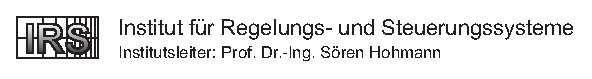
\includegraphics[width=1\textwidth]{irslogo.eps}
  \caption{Abbildung im Anhang}\label{bild_anh}
 \end{center}
\end{figure}

\section{Quellcodes}

Quellcodes lassen sich gut mit dem listings-Paket einbinden, so ist das Einbinden von entsprechend formatiertem Matlab-/C++/etc.-Code ohne Copy/Paste direkt aus der Quellcode-Datei möglich. Und hier noch ein Beispielhafter Matlab Quellcode:

\begin{lstlisting}[caption={Ein wahnsinnig komplizierter Quellcode}]
%% State Space System
asyn.SS = ss(asyn.A,asyn.B,asyn.C,asyn.D);

% Infos über das System
disp('- Informationen über das System -');
% Ordnung des Systems
asyn.n = rank(asyn.A);
disp(['Ordnung des Systems n = ', num2str(asyn.n)]);
% Polstellen
asyn.PS = pole(asyn.SS);
% Nullstellen
asyn.NS = tzero(asyn.SS);
% Beobachtbarkeit
asyn.Ob = obsv(asyn.SS);
if rank(asyn.Ob) == asyn.n
    disp('System vollständig Beobachtbar');
else
    disp('System nicht vollständig Beobachtbar');
end
% Steuerbarkeit
asyn.Os = ctrb(asyn.SS);
if rank(asyn.Os) == asyn.n
    disp('System vollständig Steuerbar');
else
    disp('System nicht vollständig Steuerbar');
end

disp('---------------------------------');
\end{lstlisting}

\end{appendix}
%% Ende des Anhangs
%% -----------------------

%%% Danksagung
%%% In Anlehnung an das IRS-Wiki zwischen Anhänge und Literatur
\ifthenelse{\boolean{symbol_english}}
{%
	%	\cleardoublepage\pdfbookmark{Acknowledgments}{acknowledgment}
	%	\ifthenelse{\boolean{symbol_english}}
{%
	\chapter*{Acknowledgments}
}
{%
	\chapter*{Danksagungen}
}
\thispagestyle{empty}

I like to acknowledge ...
}
{%
	%	\cleardoublepage\pdfbookmark{Danksagungen}{Danksagung}	% Kurzfassung den PDF Lesezeichen hinzugefügt	Manuel Schwartz 2016.02.21
	%	\ifthenelse{\boolean{symbol_english}}
{%
	\chapter*{Acknowledgments}
}
{%
	\chapter*{Danksagungen}
}
\thispagestyle{empty}

I like to acknowledge ...
}
%%%

\nocite{*} % Alle Eintr"age im Bib-File in das Literaturverzeichnis mit "ubernehmen
%\nocite{} % Nur die Eintr"age im Bib-File in das Literaturverzeichnis mit "ubernehmen die auch wirklich genutzt werden
\bibliography{bib/bibliography} % Name des BIB-Files mit den Literaturdaten %% Geaenderter Pfad, Manuel Schwartz 2015.10.13
% Empfehlenswertes Programm zum Editieren von .bib-files: JabRef, erh"altlich unter
% http://jabref.sourceforge.net/
% Direkter Link zur Version 2.2 f"ur Windows:
% http://downloads.sourceforge.net/jabref/JabRef-2.2-setup.exe

\end{document}
